%!TEX root = ./template-skripsi.tex
%-------------------------------------------------------------------------------
%                             BAB IV
%                   KESIMPULAN DAN SARAN
%-------------------------------------------------------------------------------

\chapter{HASIL DAN PEMBAHASAN}

\section{Implementasi}

\begin{figure}[H]
  \centering
  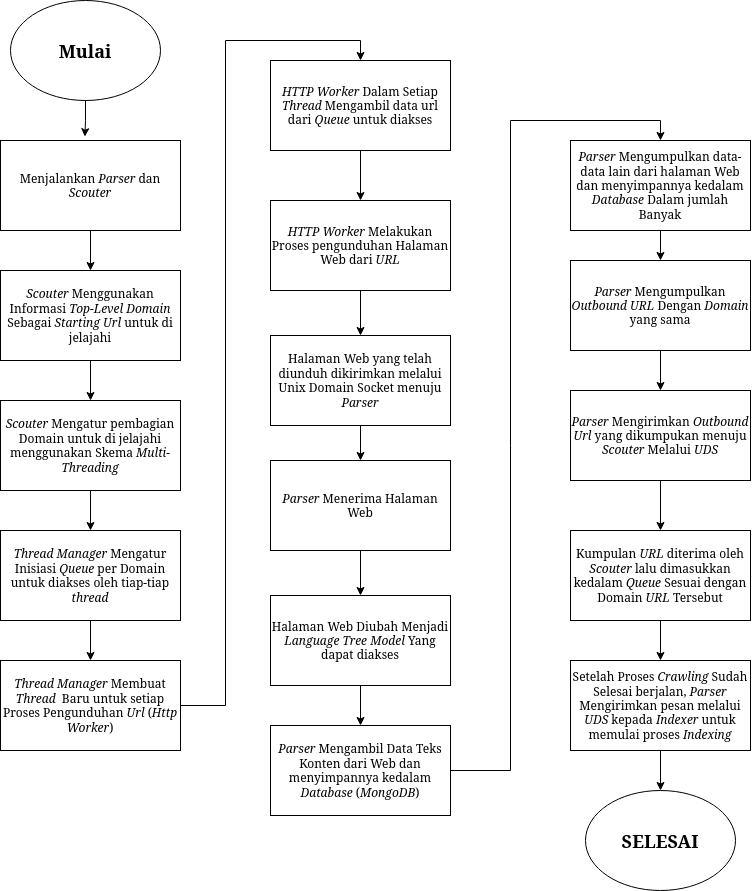
\includegraphics[keepaspectratio, width=12cm]{gambar/flowchart-penelitian.png}
  \caption{Diagram perencanaan penelitian}
  \label{gambar:flowchart_experiment}
\end{figure}

Diagram \ref{gambar:flowchart_experiment} merupakan alur tahapan penelitian yang berhasil diselesaikan, \emph{flowchart} ini merupakan penyempurnaan dari diagram perencanaan penelitan di bab 3. Secara umum terdapat dua aplikasi atau \emph{services} yang dijalankan dalam penelitian ini yaitu \emph{scouter} dan \emph{crawler} dimana \emph{scouter} bertugas sebagai penjelajah \emph{url}, pengelola akses \emph{queue} per domain, pengunduh halaman web, dan akses utama serta \emph{entry point} dari arah jalan data. \emph{Parser} sebagai pengakses \emph{HTML} dari tiap-tiap halaman web, pengambil data, dan melakukan manajemen penyimpanan data kedalam \emph{database}. Proses yang dijalankan oleh kedua \emph{services} ini berjalan secara terus menerus hingga batas waktu yang telah di tentukan dalam \emph{environment variables}.

\begin{figure}[H]
  \centering
  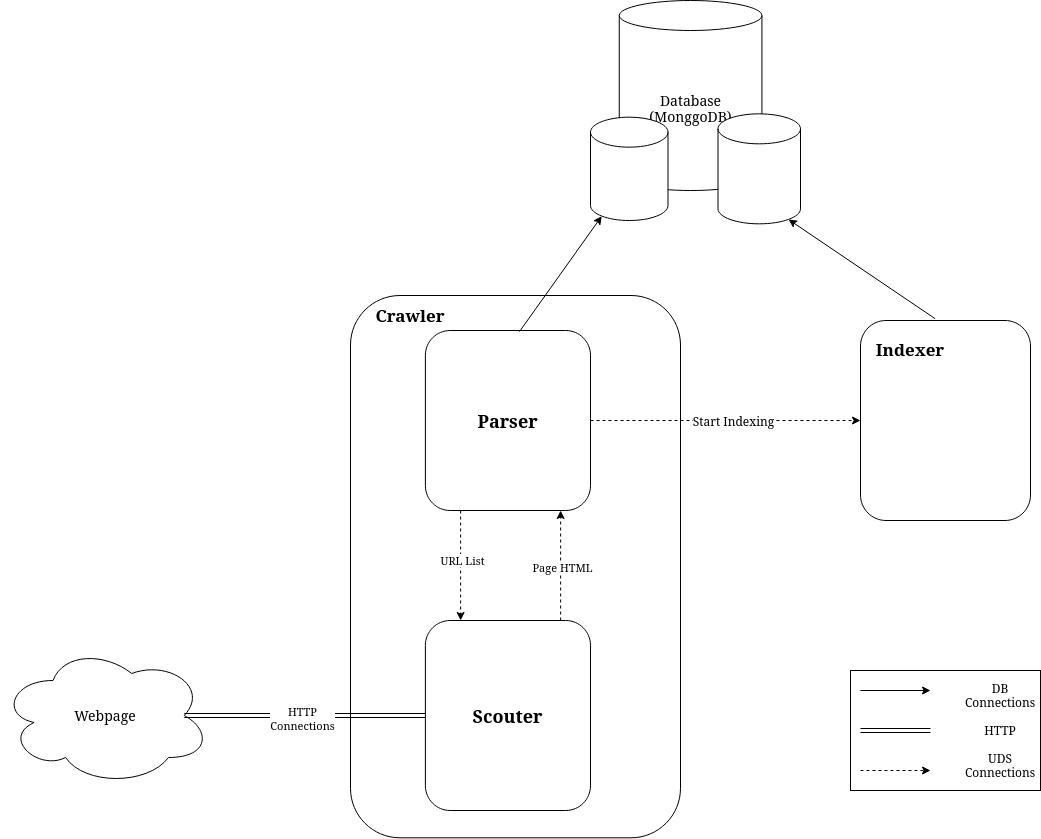
\includegraphics[keepaspectratio, width=12cm]{gambar/high-level-arch.png}
  \caption{Diagram \emph{high-level} Arsitektur Crawler}
  \label{gambar:high_level_arch}
\end{figure}

Diagram \ref{gambar:high_level_arch} merupakan gambaran umum dari arsitektur \emph{web crawler}, terdapat beberapa perbaikan dari diagram bab 3 salah satunya adalah jalur \emph{uds} kedua dari \emph{parser} menuju \emph{scouter} yang membawa \emph{outbound url} dan \emph{message} menuju \emph{indexer} yang hanya berisi \emph{start indexing}. \emph{Scouter} dan \emph{Parser} merupakan dua aplikasi atau \emph{service} bebeda yang dijalankan secara bersamaan. Untuk manajemen dua \emph{services}, menggunakan fitur \emph{workspaces} dari \emph{rust} yang memungkinkan untuk melakukan manajemen dua \emph{source code} dalam satu konteks project.

\begin{figure}[H]
  \centering
  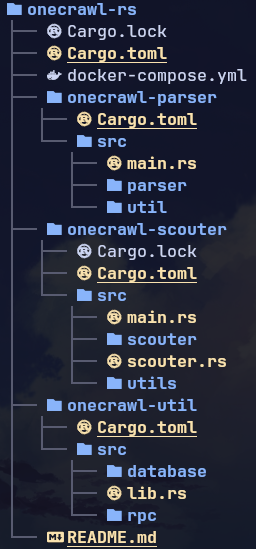
\includegraphics[keepaspectratio, width=5cm]{gambar/project_workspaces.png}
  \caption{Arsitektur penempatan \emph{file} \emph{crawler} seluruh \emph{workspaces}}
  \label{gambar:project_workspaces_arch}
\end{figure}

Gambar \ref{gambar:project_workspaces_arch} merupakan struktur arsitektur keseluruhan \emph{workspaces} dari \emph{web crawler}. Dari gambar \ref{gambar:project_workspaces_arch} dapat dilihat terdapat tiga bagian \emph{workspaces} yaitu \emph{onecrawl-scouter} sebagai \emph{scouter}, \emph{onecrawl-parser} sebagai \emph{parser}, dan \emph{onecrawl-util} sebagai \emph{custom library} yang digunakan oleh kedua \emph{services} tersebut.

\begin{figure}[H]
  \centering
  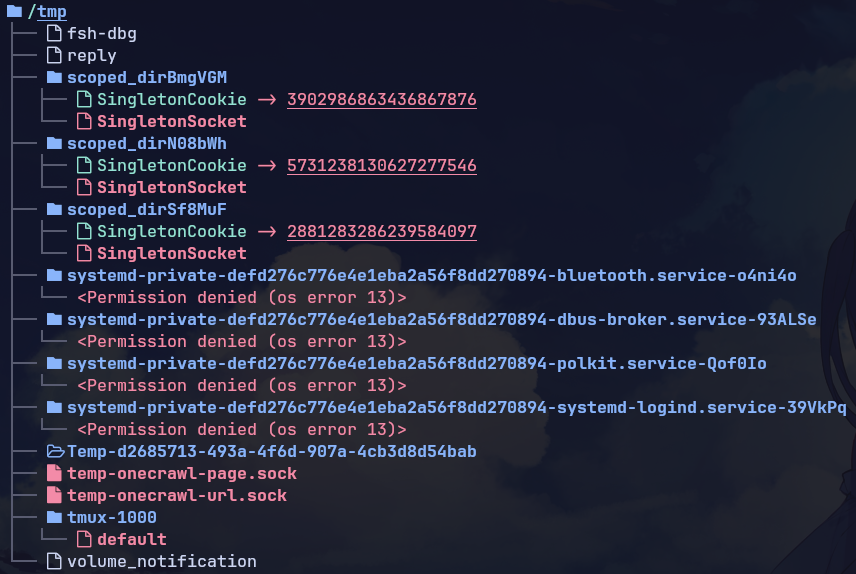
\includegraphics[keepaspectratio, width=10cm]{gambar/uds_pipe_file.png}
  \caption{Dua \emph{file} yang merupakan jalur \emph{Unix Domain Socket} dalam \emph{crawler}}
  \label{gambar:uds_pipe_file}
\end{figure}

Sebagai Jalur komunikasi antar \emph{services}, \emph{Unix Domain Socket} atau \emph{UDS} perlu sebuah file dalam direktori \emph{file} \emph{/tmp} sebagai jalur atau \emph{pipeline} dari pesan-pesan yang dikirimkan. Dalam gambar \ref{gambar:uds_pipe_file} terdapat dua file, \emph{temp-onecrawl-page.sock} sebagai \emph{placeholder} jalur komunikasi dari \emph{scouter} menuju \emph{parser} dan \emph{temp-onecrawl-url.sock} sebagai \emph{placeholder} jalur komunikasi dari \emph{parser} menuju \emph{scouter}.

\subsection{Implementasi algoritma \emph{Breadth-first Search} Modifikasi}

Implementasi algoritma \emph{breadth-first search} termodifikasi dilakukan di kedua \emph{services}, dikarenakan \emph{control flow} untuk akses halaman web berada di \emph{scouter} dan mekanisme pengumpul \emph{url} berada di \emph{parser}. Algoritma \emph{breadth-first search} termodifikasi terdiri dari dua bagian, bagian pengalokasian \emph{thread} terisolasi untuk setiap akses domain dan bagian \emph{filtering} dari \emph{url} yang dikumpulkan agar hanya sesuai dengan \emph{domain} dari halaman web tersebut.

Pembagian tiap domain pertama dilakukan saat \emph{crawler} mulai berjalan pertama kali setelah mengambil \emph{origin url} dari \emph{environment variable}. Dikarenakan setiap \emph{origin url} memiliki domain yang berbeda, tiap \emph{origin url} ini di-\emph{assign} ke \emph{thread} terisolasi masing-masing, yang dimana tiap \emph{thread} tersebut memilki \emph{queue}, \emph{thread id}, dan \emph{domain id} masing-masing sebagai \emph{identifier}.

\begin{figure}[H]
  \centering
  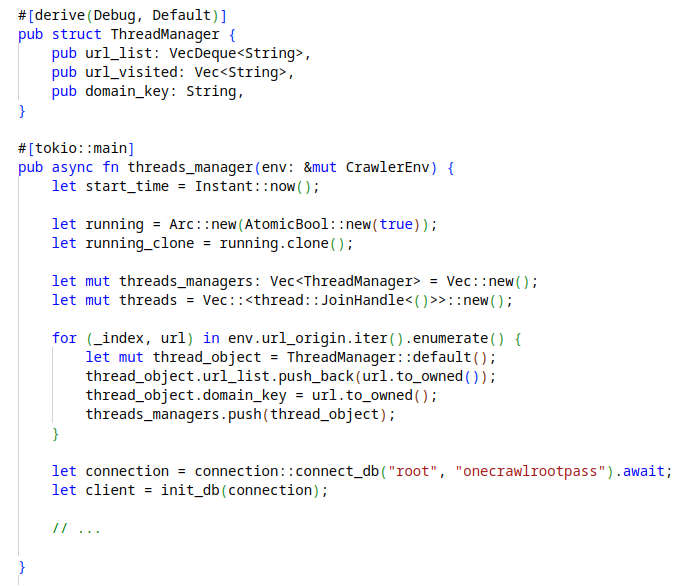
\includegraphics[keepaspectratio, width=10cm]{gambar/code-thread-manager-init.png}
  \caption{Fungsi inisiasi \emph{thread manager} sebagai aktor pengalokasi \emph{thread} untuk masing-masing domain}
  \label{gambar:thread-manager-start-bfs}
\end{figure}

Saat proses \emph{parsing} pengumpulan \emph{url} di \emph{parser} dan sebelum \emph{url list} ini dikirimkan melalui \emph{unix socket}, terlebih dahulu di-\emph{filter} \emph{url} mana yang akan dikirim. Meknaisme \emph{filtering} dilakukan dengan membandingkan \emph{outbound u.rl} yang di dapat dengan \emph{domain} dari halaman web yang sedang di \emph{parse}, bila sama maka \emph{url} dimasukkan kedalam \emph{list} bila tidak maka \emph{url} akan dihiraukan. \emph{Url} di cek per iterasi menggunakan methode \emph{map} seperti di gambar \ref{gambar:parse-link-filtering}

\begin{figure}[H]
  \centering
  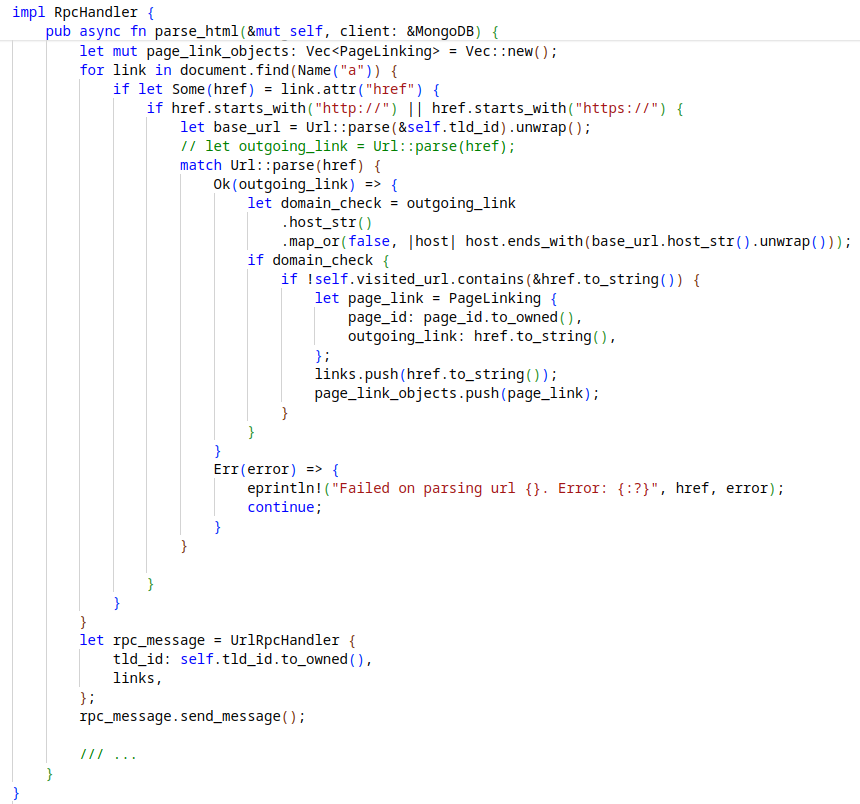
\includegraphics[keepaspectratio, width=12cm]{gambar/parse-link-gathering.png}
  \caption{Bagian kode \emph{parsing} yang melakukan \emph{filtering} terhadap url yang dikumpulkan}
  \label{gambar:parse-link-filtering}
\end{figure}

Mekanisme pembagian tiap domain pada gambar \ref{gambar:thread-manager-start-bfs} hanya dilakukan sekali saja saat \emph{startup}. Ketika \emph{scouter} sedang berjalan dan menerima \emph{incoming url} dari \emph{parser}, \emph{scouter} melakukan pengecekan terhadap pesan masuk tersebut untuk menentukan \emph{list of url} yang masuk berasal dari halaman web dengan \emph{domain} apa. \emph{List or url} tersebut di tambahkan kedalam \emph{queue} yang \emph{domain}-nya sesuai dengan \emph{domain id} dari pesan tersebut.

\begin{figure}[H]
  \centering
  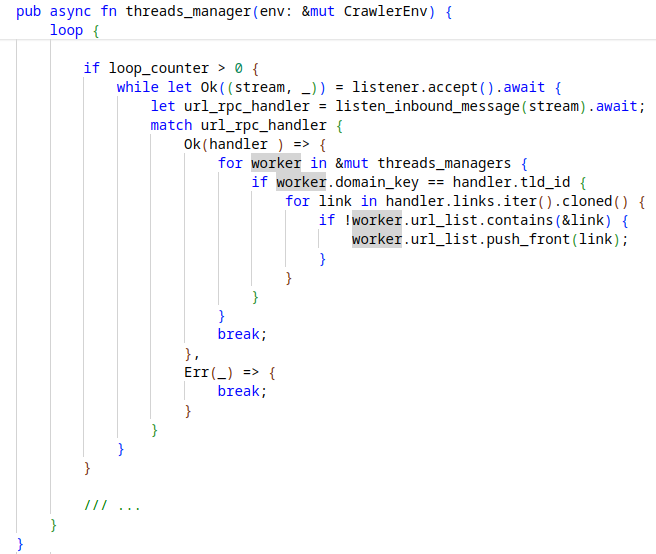
\includegraphics[keepaspectratio, width=12cm]{gambar/scouter-listen-links.png}
  \caption{Bagian kode untuk membagi url kedalam masing-masing \emph{thread}}
  \label{gambar:scouter-listen-bfs}
\end{figure}

\subsection{\emph{Scouter Service}}

\begin{figure}[H]
  \centering
  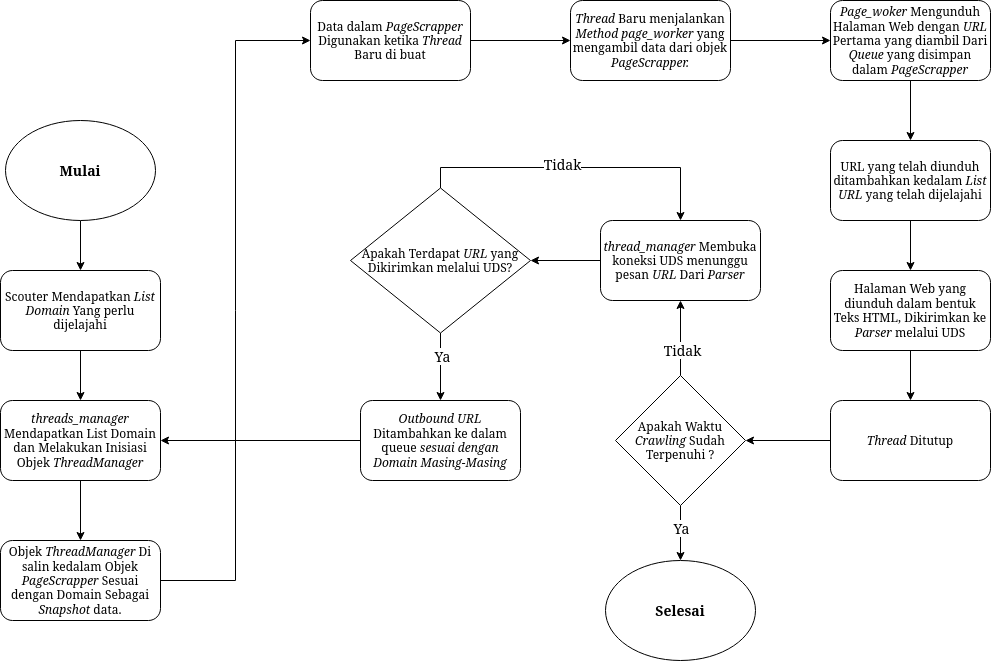
\includegraphics[keepaspectratio, width=10cm]{gambar/scouter-flowchart.png}
  \caption{\emph{Flowchart} dari mekanisme jalannya \emph{scouter service}}
  \label{gambar:scouter-flowchart}
\end{figure}

\emph{Scouter} sebagai \emph{services} yang bertugas sebagai \emph{entry point}, manajemen akses \emph{crawler} dalam menjelajahi halaman web, kontrol terhadap algoritma \emph{breadth-first search} termodifikasi, \emph{thread manager}, dan pengunduh halaman web kedalam bentuk teks \emph{HTML}. \emph{Scouter} secara umum bertugas mendapatkan daftar \emph{origin url} yang perlu dijelajahi, memasukkannya kedalam \emph{queue} per \emph{top-level domain}, mengakses \emph{url-url} tersebut menggunakan \emph{HTTP Call}, mengirimkan halaman web yang telah diunduh melalui \emph{Unix Domain Socket}, dan membuka koneksi \emph{UDS} dari \emph{parser} yang berisi daftar \emph{outbound url} yang dikumpulkan oleh \emph{parser} dari satu halaman.

\begin{figure}[H]
  \centering
  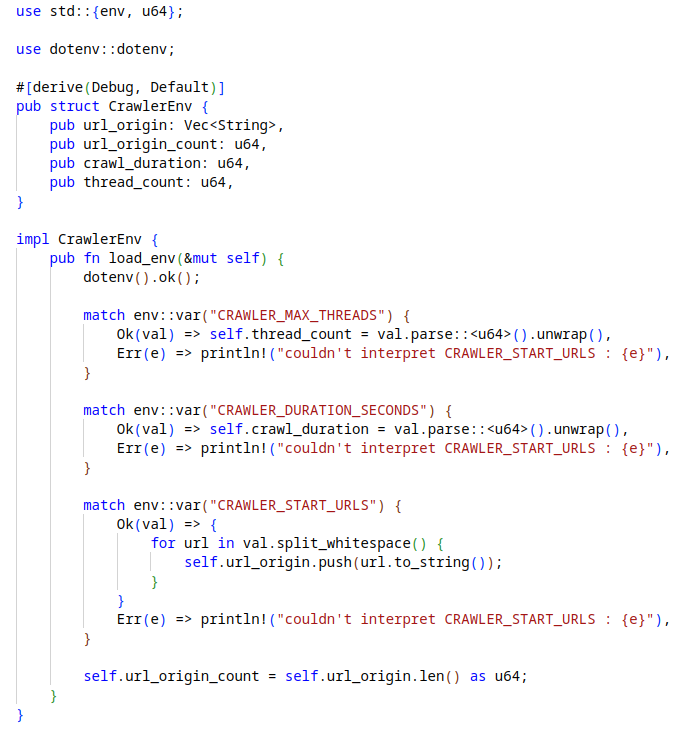
\includegraphics[keepaspectratio, width=13cm]{gambar/get_env_code.png}
  \caption{Fungsi \emph{load\_env} dalam \emph{scouter service} yang berfungsi untuk mendapatkan daftar \emph{url} dari \emph{environment variable}}
  \label{gambar:get_env_code}
\end{figure}

Diagram \ref{gambar:scouter-flowchart} menggambarkan alur keseluruhan dari \emph{scouter}. Daftar domain yang perlu dijelajahi didapatkan dari \emph{environment variables} yang disimpan dalam file \emph{.env}, variable yang disimpan adalah \emph{CRAWLER\_MAX\_THREADS}, \emph{CRAWLER\_DURATION\_SECONDS}, dan \emph{CRAWLER\_START\_URLS}. Gambar \ref{gambar:get_env_code} merupakan mekanisme dari \emph{scouter} dalam mendapatkan daftar \emph{environment variables} kedalam kode. Semua variable tesebut disimpan kedalam \emph{struct} bernama \emph{CrawlerEnv}. Untuk menjalankan mekanisme ini \emph{scouter} hanya perlu membuat objek dengan tipe data \emph{CrawlerEnv} dan memanggil fungsi \emph{load\_env} untuk mengisi objek tersebut dengan \emph{environment variables}. Gambar \ref{gambar:load_env-called} merupakan contoh kode saat fungsi \emph{load\_env()} dipanggil dan mengisi objek \emph{env} yang berisi \emph{environment variables}.

\begin{figure}[H]
  \centering
  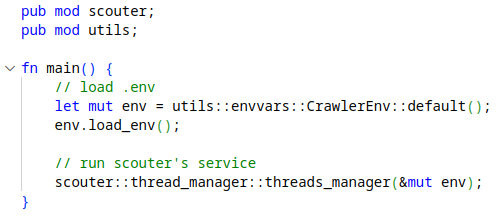
\includegraphics[keepaspectratio, width=10cm]{gambar/load_env_called.png}
  \caption{Pemanggilan fungsi \emph{load\_env} dalam fungsi \emph{main()}}
  \label{gambar:load_env-called}
\end{figure}

Kode dalam gambar \ref{gambar:load_env-called} juga menunjukkan objek \emph{env} dipindahkan sebagai paramter dari fungsi \emph{threads\_manager}. Fungsi \emph{threads\_manager} merupakan fungsi utama yang menjalankan fungsionalitas \emph{scouter}.

\begin{figure}[H]
  \centering
  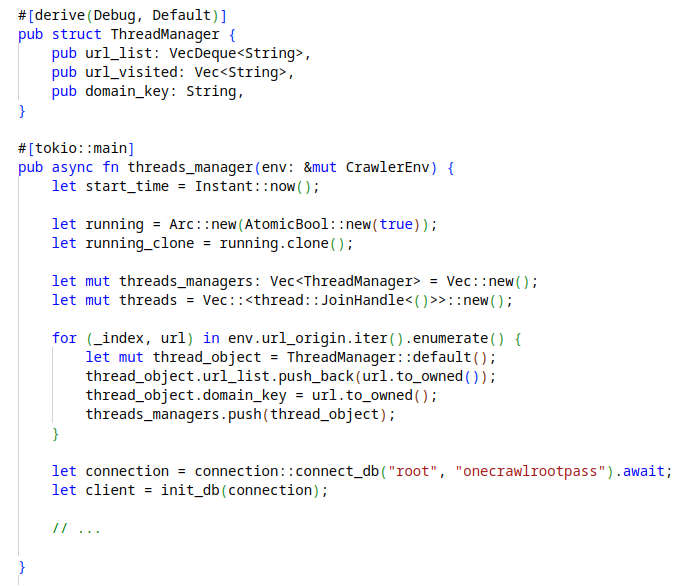
\includegraphics[keepaspectratio, width=10cm]{gambar/code-thread-manager-init.png}
  \caption{Bagian dari fungsi \emph{thread\_manager} yang berfungsi sebagai inisiasi mekanisme \emph{multi-threading}}
  \label{gambar:thread-manager-func-init}
\end{figure}

Gambar \ref{gambar:thread-manager-func-init} merupakan bagian kode dari fungsi \emph{thread\_manager()} dan definisi \emph{struct} \emph{ThreadManager}. Fungsi \emph{thread\_manager()} merupakan fungsi yang mengatur \emph{resource allocation}, menunggu \emph{inbound message} dari \emph{parser}, dan mekanisme pembuatan \emph{thread} baru. Dalam gambar \ref{gambar:thread-manager-func-init} fungsi \emph{thread\_manager()} terlihat melakukan inisiasi \emph{start\_time} yang digunakan untuk mencatat waktu dimulainya proses dan beberapa variable lain yang digunakan untuk \emph{resource allocation} per operasi pengunduhan halaman web. Kode ini juga membuat variable baru yang bernama \emph{thread\_managers}, variable ini berfungsi untuk menampung satu atau lebih objek dengan tipe data \emph{ThreadManager} yang akan digunakan untuk menampung informasi-informasi yang akan digunakan dalam \emph{scope} dari masing-masing \emph{thread}.

\begin{figure}[H]
  \centering
  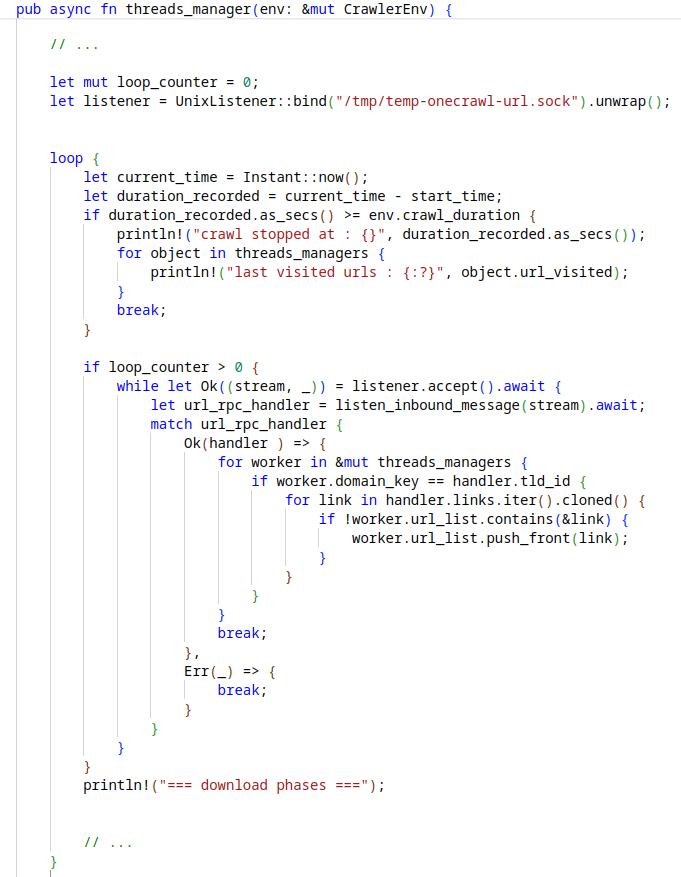
\includegraphics[keepaspectratio, width=10cm]{gambar/thread_manager-code-loop.png}
  \caption{Bagian kode yang bertugas untuk inisiasi \emph{infinite loop} dan mendeteksi \emph{incoming message} dari \emph{parser service}}
  \label{gambar:code-loop-thread-manager}
\end{figure}

Fungsi \emph{thread\_manager()} juga menjalankan peran sebagai pengatur mekanisme algoritma \emph{breadth-first search} yang digunakan oleh \emph{scouter}, dikarenakan \emph{scouter} ini harus berjalan terus menerus hingga waktu habis maka fungsi \emph{thread\_manager()} harus menjalankan \emph{infinite loop} yang berhenti hanya jika waktu jalannya \emph{scouter} telah terpenuhi. Selain mekanisme \emph{spawn thread}, dalam gambar \ref{gambar:code-loop-thread-manager} juga terdapat kode untuk mendengar \emph{inbound message} dengan melakukan bind dengan \emph{socket file} \emph{/tmp/temp-onecrawl-url.sock}. Fungsi \emph{listen\_inbound\_message()} merupakan fungsi untuk menerima \emph{inbound message} tersebut dan mengembalikan objek yang berisi \emph{message} yang telah di \emph{parse}.

\begin{figure}[H]
  \centering
  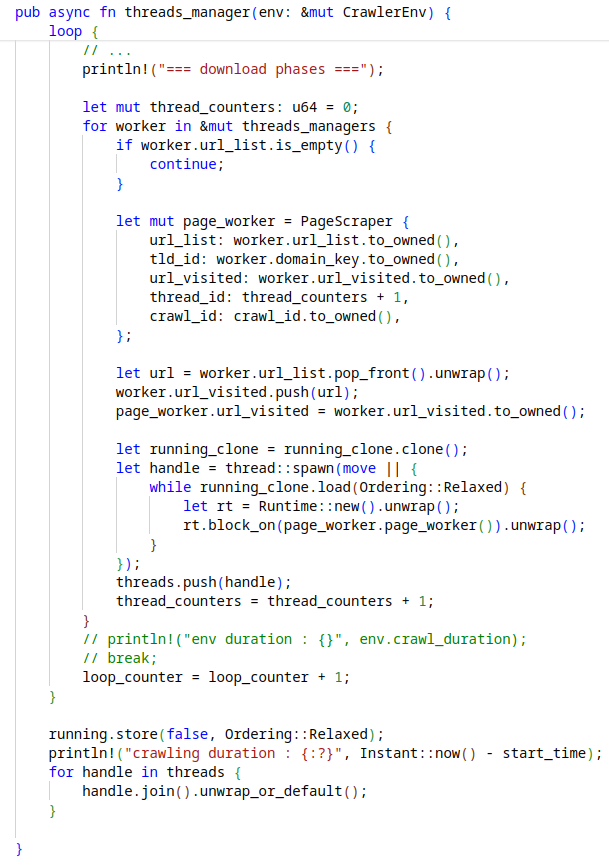
\includegraphics[keepaspectratio, width=10cm]{gambar/thread_manager_spawn_code.png}
  \caption{Bagian kode dari fungsi \emph{thread\_manager} yang berfungsi untuk \emph{spawning thread} tiap \emph{url} masuk}
  \label{gambar:thread-manager-spawn-code}
\end{figure}

Dalam setiap iterasi \emph{loop}, \emph{scouter} menjalankan proses pengunduhan dalam \emph{thread} yang terisolasi. Untuk menghindari komplikasi waktu dari proses \emph{locking} dan \emph{race condition} saat \emph{dequeue} setiap thread memiliki \emph{queue} masing-masing. Untuk menghentikan semua proses dalam \emph{thread} yang sedang berjalan secara \emph{graceful} menggunakan \emph{atomic variable} bernama \emph{running}, saat \emph{thread} baru dibuat, setiap \emph{thread} berjalan dengan konteks \emph{Ordering::relaxed} dan proses dalam \emph{threads} hanya akan berjalan jika \emph{Ordering::relaxed} bernilai benar atau \emph{true}. Dengan mekanisme ini kode dapat di kustomisasi sehingga bila sejumlah waktu telah dicapai, variable \emph{running} dapat diubah statusnya dari \emph{Ordering::relaxed} dengan status \emph{true} menjadi \emph{false}, ini akan memicu mekanisme dalam \emph{thread} untuk berhenti.

\begin{figure}[H]
  \centering
  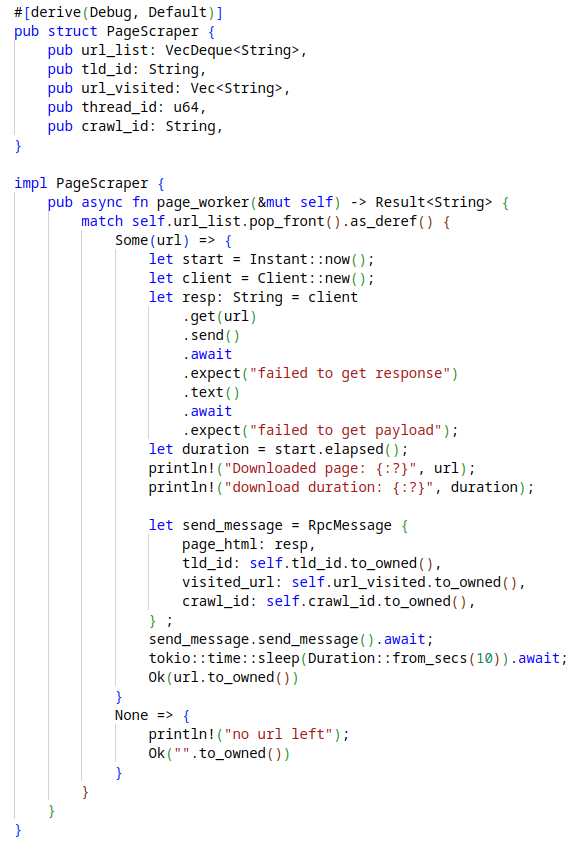
\includegraphics[keepaspectratio, width=10cm]{gambar/page_worker-code.png}
  \caption{ Fungsi \emph{page\_worker} untuk melakukan pengunduhan halaman web}
  \label{gambar:page-worker-code}
\end{figure}

Dari gambar \ref{gambar:thread-manager-spawn-code} dapat dilihat didalam \emph{thread} yang telah dibuat terjadi pemanggilan metode \emph{page\_worker} yang merupakan modul utama pemanggilan \emph{http} dalam \emph{scouter service} , metode ini adalah metode dari objek \emph{page\_woker} yang sudah di buat sebelumnya dan bekerja sebagai fungsi utama yang dieksekusi didalam masing-masing \emph{thread} yang terisolasi. Gambar \ref{gambar:page-worker-code} merupakan potongan kode dari definisi \emph{class} \emph{PageScrapper} yang merupakan \emph{blueprint} dari objek \emph{page\_worker} dan fungsi \emph{page\_worker} itu sendiri. Dari gambar \ref{gambar:page-worker-code} dapat terlihat bahwa fungsi \emph{page\_worker} hanya melakukan dua hal utama yaitu, proses pengunduhan teks \emph{html} dari halaman web dan mengirimkan teks tersebut beserta informasi pendukung lainnya melalui \emph{send\_message}. Objek \emph{raw\_page\_mes} dibuat berdasarkan \emph{class} \emph{RpcMessage}. Fungsi \emph{page\_worker} ini memberikan \emph{return value} \emph{url} yang telah dijelajahi dan status apakah fungsi berhasil dijalankan atau tidak. Gambar \ref{gambar:scouter-flowchart} merupakan gambaran secara umum bagaimana fungsi ini berjalan.

\begin{figure}[H]
  \centering
  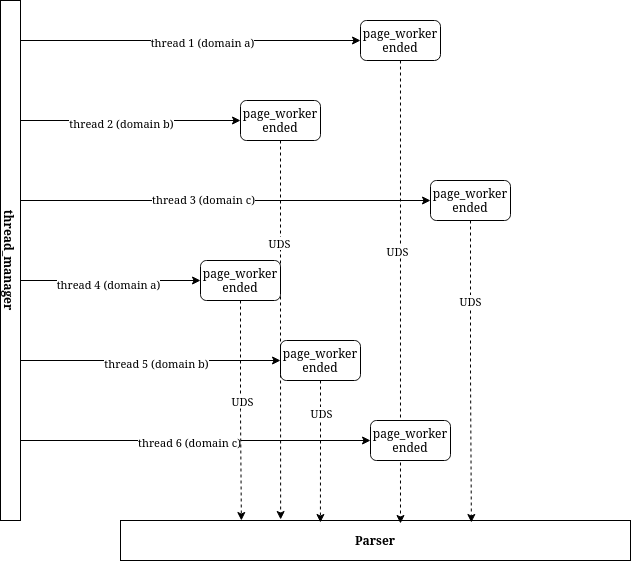
\includegraphics[keepaspectratio, width=10cm]{gambar/scouter-multithread-diagram.png}
  \caption{Diagram mekanisme \emph{multi-thread} dari \emph{scouter service}}
  \label{gambar:scouter-multithread-diagram}
\end{figure}

\subsection{Komunikasi pengiriman \emph{page} melalui \emph{Unix Domain Socket}} 

Seperti yang ditunjukkan dalam kode di gambar \ref{gambar:page-worker-code} dan diagram dari gambar \ref{gambar:scouter-multithread-diagram} teks \emph{HTML} hasil pengunduhan \emph{scouter}, selanjutnya dikirimkan kepada \emph{parser services} melalui \emph{Unix Domain Socket} atau \emph{UDS}. Proses pengiriman teks ini dilakukan secepatnya setelah proses pengunduhan selesai. Agar parser dapat membaca pesan dengan mudah, struktur \emph{class} dari pesan pada \emph{scouter service} dan \emph{parser service} menggunakan \emph{class} yang sama dan pesan di kirim dalam bentuk \emph{json string}.

\begin{figure}[H]
  \centering
  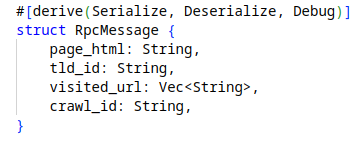
\includegraphics[keepaspectratio, width=10cm]{gambar/rpc-message-struct.png}
  \caption{Struktur dari pesan \emph{rpc} yang dikirimkan}
  \label{gambar:rpc-struct-scouter}
\end{figure}

Konten pesan yang dikirimkan tidak hanya berisi teks \emph{html} dari halaman yang diunduh tetapi juga \emph{top-level domain} dari halaman tersebut, \emph{visited url} yang telah dijelajahi sampai saat halaman tersebut di unduh, dan \emph{crawl id} dari halaman tersebut.

\begin{figure}[H]
  \centering
  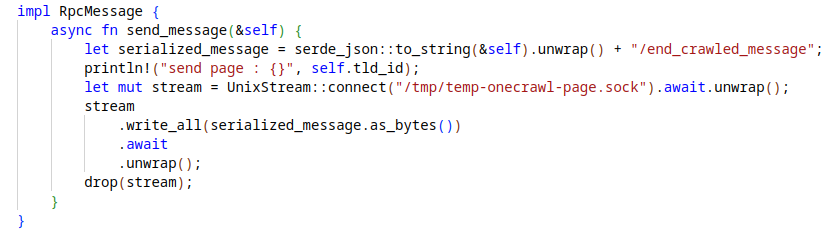
\includegraphics[keepaspectratio, width=13cm]{gambar/rpc-send-message-scouter.png}
  \caption{Fungsi yang mengirim \emph{rpc} message}
  \label{gambar:rpc-send-message-scouter}
\end{figure}

Fungsi \emph{send\_message()} yang terdapat di gambar \ref{gambar:rpc-send-message-scouter} merupakan fungsi untuk mengirim \emph{message} yang di buat sebelumnya melalui koneksi \emph{Unix Domain Socket}. Sebelum pesan dikirimkan pesan tersebut di serialisasi menjadi bentuk \emph{json binary} terlebih dahulu lalu dikirimkan menggunakan metode \emph{write\_all}, melalui jalur \emph{socket} \emph{/tmp/temp-onecrawl-page.sock}. Pesan yang sudah dikirimkan dikirimkan ini nantinya akan diterima oleh \emph{parser service} untuk di proses.


\subsection{\emph{Parser Service}}

\emph{Parser} merupakan \emph{services} yang bertugas sebagai pengekstrak data dan penyimpan data dari halaman-halaman web yang telah diunduh oleh \emph{scouter services}. Halaman web yang sudah berbentuk teks didapatkan oleh \emph{parser} dari \emph{scouter sevices} melalui \emph{uds messages}, data mentah yang didapatkan dari \emph{uds messages} berbentuk \emph{json binary} yang kemudian akan di \emph{deserialize} menjadi suatu \emph{object}. \emph{Object} tersebut yang selanjutnya akan diproses lebih lanjut dan teks \emph{html} yang ada didalam objek tersebut di-\emph{parse} dan diambil data-datanya. Data yang didapat ini yang dimasukkan kedalam \emph{databases}.

\begin{figure}[H]
  \centering
  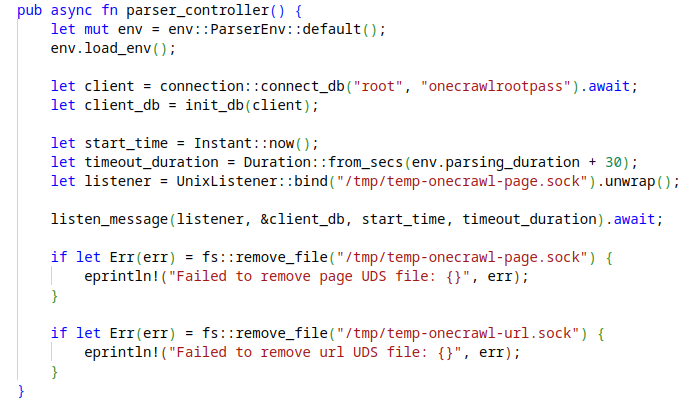
\includegraphics[keepaspectratio, width=13cm]{gambar/parser-controller-code.png}
  \caption{Bagian kode fungsi \emph{parser\_controller} sebagai \emph{entry point} dari \emph{parser services}}
  \label{gambar:parser-controller}
\end{figure}

Fungsi \emph{parser\_controller()} dari gambar \ref{gambar:parser-controller} merupakan \emph{entry point} dari jalannya seluruh proses dalam \emph{parser service}. Hal pertama yang dilakukan dalam fungsi ini adalah membuka koneksi kedalam \emph{database}, selain itu fungsi ini juga menginisiasi \emph{timestamp} untuk menghitung waktu jalannya \emph{parser} dan inisiasi koneksi \emph{socket}. Proses \emph{binding port} dilakukan di fungsi ini ketika fungsi \emph{bind()} dipanggil, hasil dari funsi itu adalah \emph{listener address} yang dapat digunakan untuk menerima \emph{message} dari \emph{unix domain socket}. Fungsi \emph{listen\_message()} yang dipanggil di dalam \emph{parser\_controller()} merupakan fungsi utama yang menjalankan proses \emph{listening} dari \emph{socket}. Setelah semua mekanisme \emph{parser} selesai \emph{parser\_controller()} akan menghapus dua \emph{file socket} yang telah di buat.

\begin{figure}[H]
  \centering
  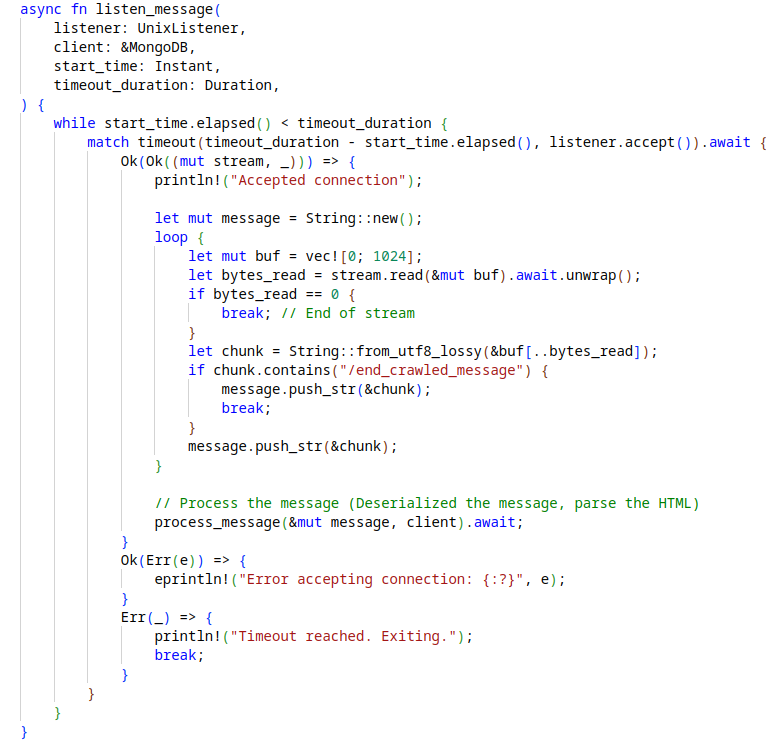
\includegraphics[keepaspectratio, width=13cm]{gambar/parser-listen-message.png}
  \caption{Funsgi \emph{listen\_message} sebagai manajemen \emph{timout} mekanisme \emph{listening} untuk pesan masuk dari \emph{scouter}}
  \label{gambar:parser-listen-message}
\end{figure}

Fungsi \emph{listen\_message()} dari gambar \ref{gambar:parser-listen-message} memuat mekanisme \emph{timout} dari parser, singkatnya dikarenakan proses \emph{binding} dari \emph{port} berada di \emph{parser} makan \emph{service} ini perlu dijalankan lebih dahulu dibanding \emph{scouter}. Untuk menghindari inkonsistensi dalam penggunaan \emph{port} yang disebabkan \emph{parser} juga yang menghapus dua file \emph{port} seperti di gambar \ref{gambar:parser-controller} , maka \emph{parser} harus berhenti beberapa detik setelah \emph{scouter} berhenti, ini dapat dicapai dengan menambah batasan waktu selama 30 detik. Selain mekanisme \emph{timeout}, \emph{listen\_message()} juga melakukan \emph{processing} terhadap \emph{binary} dari pesan yang diterima dengan mengubahnya menjadi \emph{string} dan mencari pembatas antar pesan yang berbentuk teks \emph{end crawled message}. Teks pesan yang sudah masuk selanjutnya langsung dipindahkan agar dapat digunakan oleh fungsi \emph{process\_message()} untuk di \emph{deseralized}.

\begin{figure}[H]
  \centering
  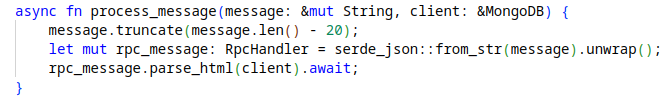
\includegraphics[keepaspectratio, width=13cm]{gambar/parser-process-message-code.png}
  \caption{Fungsi \emph{process\_message} sebagai fungsi deserialisasi pesan \emph{socket} kedalam struktur yang jelas}
  \label{gambar:parser-process-message}
\end{figure}

Fungsi \emph{process\_message()} hanya bertugas untuk membersihkan dan melakukan \emph{deserialized} data mentah dari \emph{socket} kedalam objek yang terstruktur, di dalam fungsi ini juga akan dipanggil metode \emph{parse\_html()} fungi ini yang akan melakukan sebagian besar operasi pengambilan data dari halaman web.

\begin{figure}[H]
  \centering
  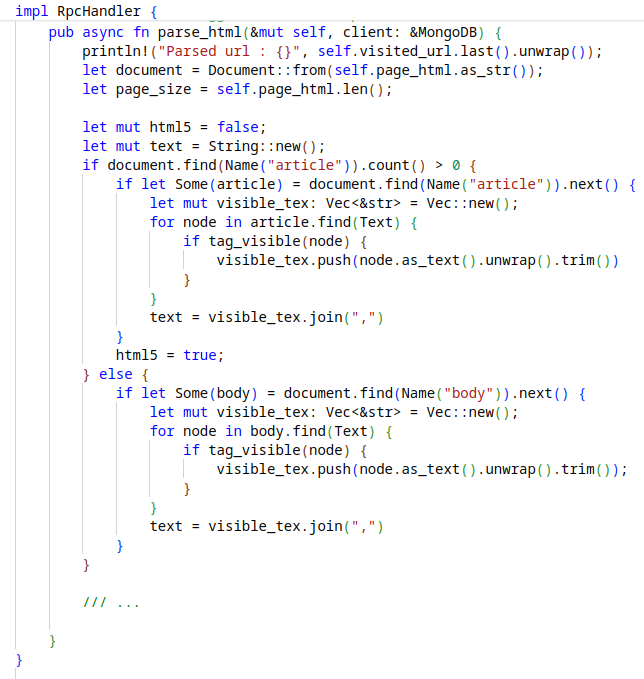
\includegraphics[keepaspectratio, width=10cm]{gambar/parse-html-body-text.png}
  \caption{Fungsi \emph{parse\_html()} sebagai fungsi utama dalam proses \emph{parsing} halaman web}
  \label{gambar:parse-html-body-text}
\end{figure}

Fungsi \emph{parse\_html()} melakukan penguraian dan pengambilan data dari halaman web yang telah diunduh. Sebelum data diambil untuk memudahkan pengambilan data dilakukan pembuatan \emph{language tree} ketika \emph{class Document} dipanggil, objek \emph{document} yang telah dibuat merupakan \emph{language tree} yang sudah jadi dan dapat dimanimulasi \emph{dom}-nya. Data yang akan diambil dikelompokkan berdasarkan jenis data dan pengaruhnya terhadap jenis informasi yang akan di ambil dari halaman web tersebut. Dalam implementasi \emph{web crawler} ini informasi yang paling penting untuk dikumpulkan adalah teks konten dalam \emph{body html}, data ini dikumpulkan untuk perhitungan \emph{rank} dari tiap-tiap halaman tersebut. Hal ini dapat terlihat di kode dalam gambar \ref{gambar:parse-html-body-text} dimana bagian kode untuk \emph{filtering} dan pengumpulan teks ini di dilakukan pertama kali. Mekanisme pengumpulan ini dilakukan oleh fungsi dengan mengumpulkan seluruh teks didalam \emph{body} dan melakukan filtering pada teks.

\begin{figure}[H]
  \centering
  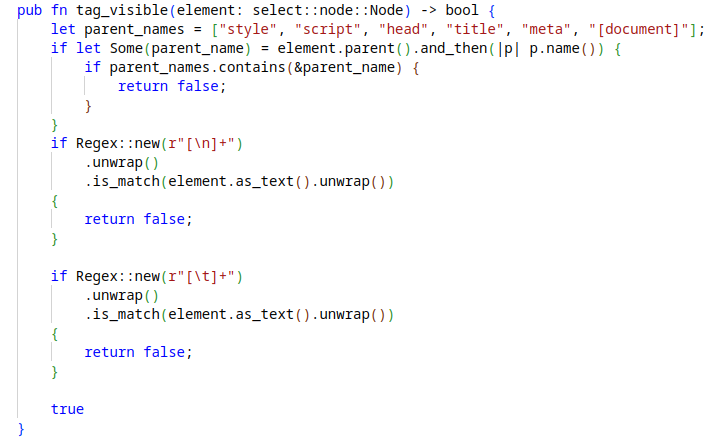
\includegraphics[keepaspectratio, width=10cm]{gambar/parser-tag-visible.png}
  \caption{Fungsi \emph{tag\_visible()} sebagai fungsi yang melakukan \emph{filtering} pada teks yang dikumpulkan}
  \label{gambar:parse-tag-visible}
\end{figure}

Proses filtering ini dilakukan oleh fungsi \emph{tag\_visible()} yang direferensikan di gambar \ref{gambar:parse-html-body-text}, fungsi ini melakukan filtering terhadap teks yang dikumpulkan. Tujuan dari proses ini adalah agar teks yang bukan konten dari halaman web tidak akan masuk kedalam \emph{database}. Teks yang disaring oleh fungsi ini dapat dilihat di kode dalam gambar \ref{gambar:parse-tag-visible} yaitu teks yang ada didalam \emph{tag} \emph{style}, \emph{script}, \emph{head}, \emph{title}, \emph{meta}, dan \emph{document}. Selain itu fungsi ini juga menyaring \emph{new line} dan \emph{new tab} yang direpresentasikan oleh karakter \emph{"n"} dan \emph{"t"} dari teks yang akan dimasukkan.

\begin{figure}[H]
  \centering
  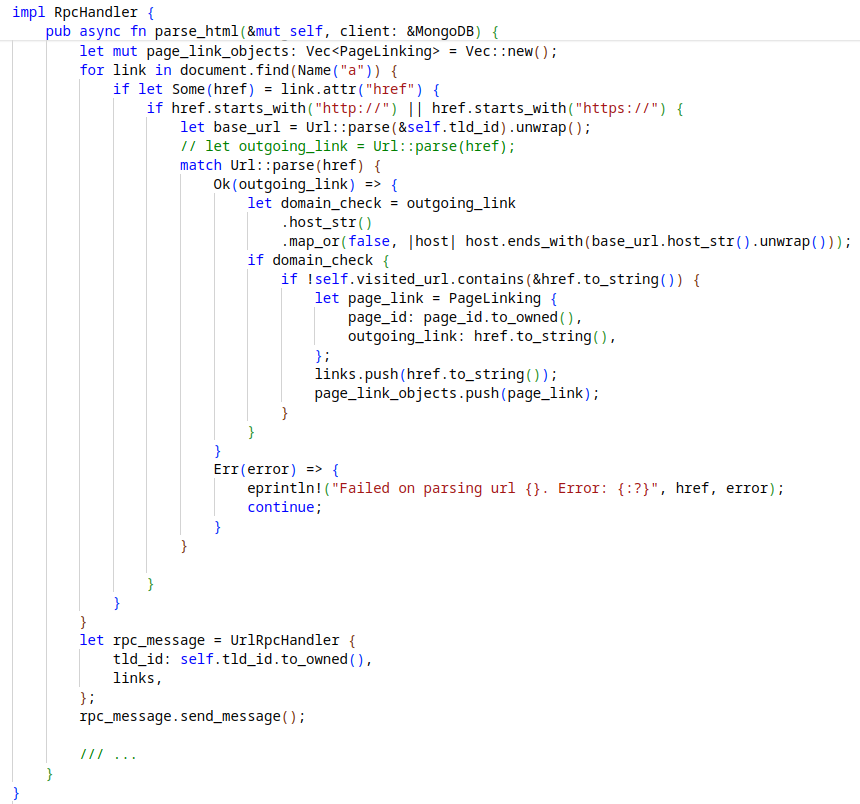
\includegraphics[keepaspectratio, width=12cm]{gambar/parse-link-gathering.png}
  \caption{Bagian kode dari fungsi \emph{parse\_html()} yang mengumpulkan \emph{outbound url} dari halaman web}
  \label{gambar:parse-link-gathering}
\end{figure}

Selain konten teks \emph{outbound url} juga perlu dikumpulkan, kumpulan \emph{url} ini perlu di saring terlebih dahulu untuk dicek apakah \emph{url} ini merujuk pada \emph{website} dengan domain yang sama atau tidak. Bila \emph{url} merujuk pada domain yang sama, maka akan dikumpulkan. Kumpulan \emph{url} ini selanjutnya akan di masukkan kedalam \emph{database} dan juga dikirimkan ke \emph{scouter service} melaui koneksi \emph{Unix Domain Socket}. \emph{Parser} juga menyimpah informasi-informasi lain seperti \emph{form}, \emph{list}, dan \emph{script} dari halaman web tersebut.

\subsection{Komunikasi balik pengiriman \emph{URL} melalui \emph{Unix Domain Socket}}

\begin{figure}[H]
  \centering
  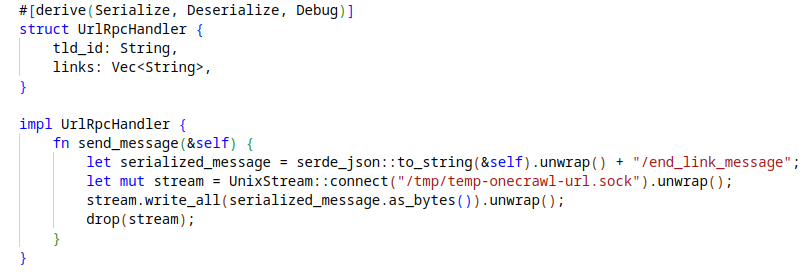
\includegraphics[keepaspectratio, width=14cm]{gambar/parser-udp-send-message.png}
  \caption{Fungsi \emph{method} dan struktur dari \emph{rpc message} yang dikirimkan oleh \emph{parser service}}
  \label{gambar:parse-send-message}
\end{figure}

Kode pada gambar \ref{gambar:parse-link-gathering} memperlihatkan dipanggilnya fungi \emph{send\_message()}, fungsi ini merupakan mekanisme \emph{parser service} untuk mengirimkan \emph{url} kepada \emph{scouter service}. Kumpulan \emph{url} ini yang akan ditambahkan ke \emph{queue} untuk diakses selanjutnya oleh \emph{scouter}. Gambar \ref{gambar:parse-send-message} merupakan definisi objek dan fungsi dari mekanisme pengiriman pesan ini. Secara general ini merupakan mekanisme yang sama dengan proses pengiriman pesan dari \emph{scouter service} dengan perbedaan pada alamat \emph{file socket} yang digunakan.

\begin{figure}[H]
  \centering
  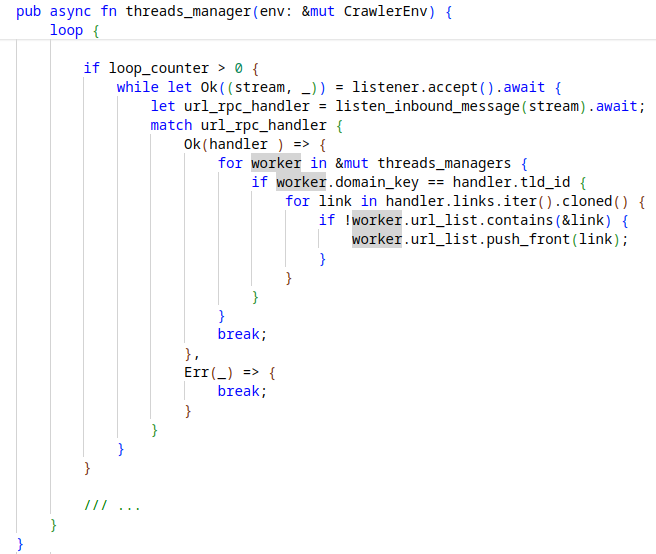
\includegraphics[keepaspectratio, width=14cm]{gambar/scouter-listen-links.png}
  \caption{Bangian kode dalam \emph{scouter service} yang menerima \emph{rpc message} dari \emph{parser service}}
  \label{gambar:scouter-listen-link}
\end{figure}

Pesan yang sudah dikirimkan oleh \emph{parser} diterima oleh \emph{scouter}, mekanisme \emph{scouter} dalam menerima pesan ini adalah dengan mengumpulkan \emph{url} yang didapatkan dari \emph{socket}, mencocokkannya dengan \emph{top level domain} yang ada di dalam \emph{scouter} dan menyimpannya kedalam \emph{queue} yang sesuai dengan \emph{domain} tersebut, seperti yang terlihat di kode dalam gambar \ref{gambar:scouter-listen-link}.

\subsection{Penyimpanan data dari \emph{Parser} dan model data \emph{Databases}}

Data-data yang sudah dikumpulkan oleh parser seperti teks konten, judul, \emph{form}, \emph{list} dan, lainnya seluruhnya di masukkan kedalam database dengan nama \emph{collection} yang sesuai jenis data tersebut. Data seperti teks konten, judul, dan deskripsi halaman web disimpan dalam \emph{collection} yang bernama \emph{page\_information}, sedangkan informasi yang berhubungan dengan \emph{url} disimpan dalam \emph{page\_links collection} dan seterusnya.

\begin{figure}[H]
  \centering
  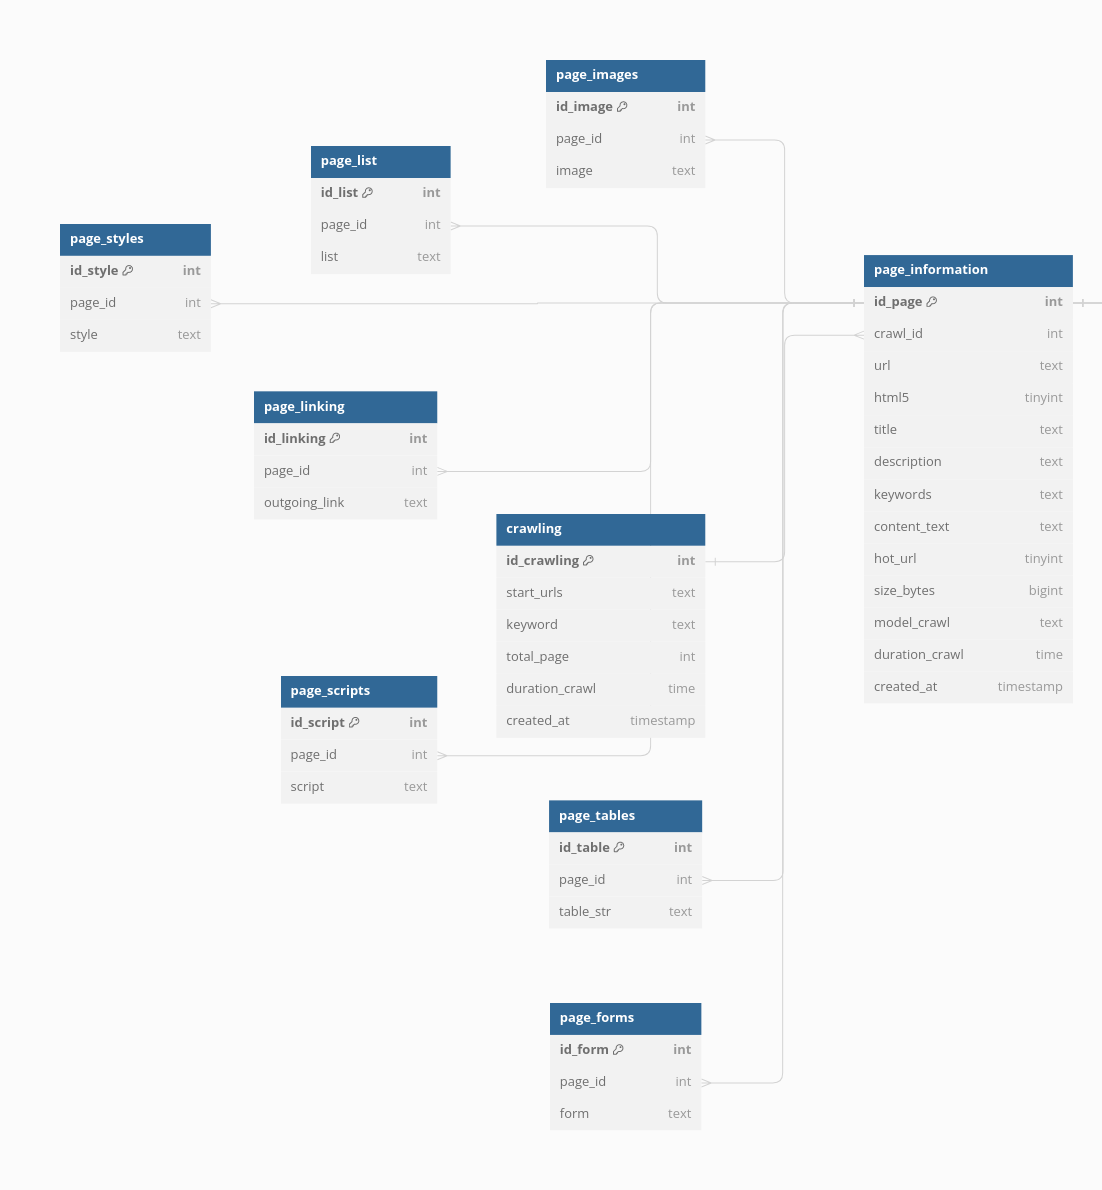
\includegraphics[keepaspectratio, width=14.5cm]{gambar/crawler-erd.png}
  \caption{\emph{Entity Relations Diagram} untuk database crawler}
  \label{gambar:erd-crawler}
\end{figure}

Dari gambar \ref{gambar:erd-crawler} dapat dilihat bahwa \emph{id} dari \emph{page\_information} digunkana sebagai \emph{foreign key} di dalam \emph{collection}, karena satu halaman web hanya akan memiliki satu \emph{page\_information} maka masuk akal untuk menjadikan \emph{id} tersebut sebagai \emph{key identifier} di dalam \emph{collection} lain. \emph{Primary key} atau id dari \emph{page\_information} didapat langsung setelah proses \emph{insert} dan disimpan dalam variabel \emph{page\_id}. Variabel ini yang selanjutnya akan digunakan terus menerus ketika proses penyimpanan data

\begin{figure}[H]
  \centering
  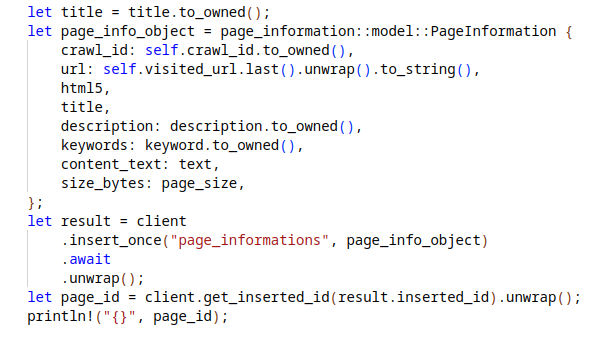
\includegraphics[keepaspectratio, width=11cm]{gambar/insert-page-info.png}
  \caption{Bagian kode yang berfungsi untuk memasukkan \emph{page\_information} kedalam \emph{database}}
  \label{gambar:insert-page-info}
\end{figure}

Untuk data-data yangh jumlah nya banyak seperti \emph{url}, \emph{script}, \emph{table}, \emph{list}, \emph{image}, \emph{form}, dan \emph{style} metode penyimpanan yang digunakan adalah \emph{insert\_bulk()} seperti dalam kode di gambar \ref{gambar:bulk-insert} agar seluruh data disimpan sekaligus tanpa menggunakan mekanisme \emph{looping}. Ini akan mempercepat proses penyimpanan data terutama pada halaman web yang memiliki jumlah data yang banyak.

\begin{figure}[H]
  \centering
  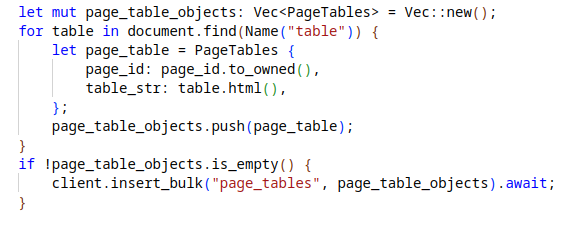
\includegraphics[keepaspectratio, width=10cm]{gambar/bulk-insert-code.png}
  \caption{Contoh pemanggilan fungsi \emph{bulk\_insert()} untuk memasukkan lebih dari satu data sekaligus}
  \label{gambar:bulk-insert}
\end{figure}

\subsection{\emph{Shared Utility Library}}

\emph{Onecrawl-util} merupakan \emph{shared library} yang di-digunakan oleh \emph{scouter service} dan \emph{parser service}. \emph{Shared Library} ini dibuat untuk memudahkan pemanggilan dan penggunaan \emph{query} terhadap database \emph{mongodb} yang digunakan di kedua \emph{services} tersebut. Fungsi yang didefinisikan dalam \emph{onecrawl util} yang dapat digunakan \emph{service} lain yaitu \emph{insert\_once()}, \emph{insert\_bulk()}, \emph{get\_inserted\_id()}, \emph{check\_value()}, dan \emph{count\_data()}.

\begin{figure}[H]
  \centering
  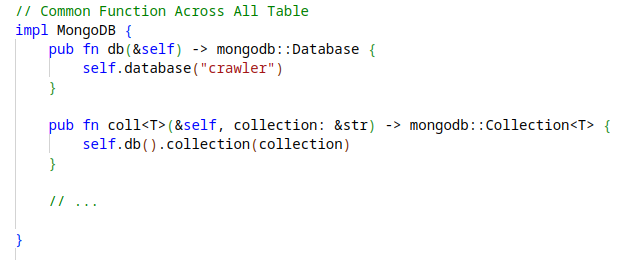
\includegraphics[keepaspectratio, width=13cm]{gambar/db-coll-func-util.png}
  \caption{Inisiasi objek \emph{database} yang akan digunakan seterusnya untuk operasi \emph{database}}
  \label{gambar:db-coll-definition}
\end{figure}

Untuk memudahkan inisiasi saat fungsi dipanggil oleh kedua \emph{services}, \emph{library} ini memiliki dua fungsi \emph{db} dan \emph{coll} yang dapat disatukan dengan \emph{chain link} pemanggilannya. Kedua fungsi ini digunakan untuk menginisiasi nama \emph{database} dan \emph{collection} serta mengeneralisasikan \emph{struct} untuk \emph{collection} yang akan berinteraksi dengan fungsi.

\begin{figure}[H]
  \centering
  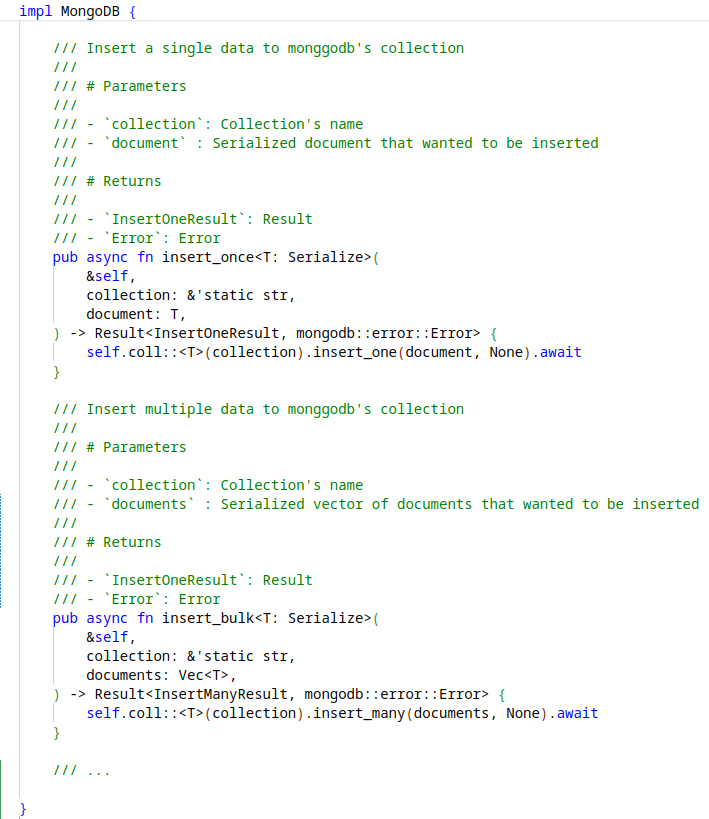
\includegraphics[keepaspectratio, width=12cm]{gambar/insert-util-code.png}
  \caption{Fungsi operasi \emph{insert} dalam \emph{shared utility library}}
  \label{gambar:insert-util-code}
\end{figure}

Fungsi \emph{insert\_once()} dan \emph{insert\_bulk()} pada gambar \ref{gambar:insert-util-code} merupakan dua fungsi yang paling sering dipanggil dalam kedua \emph{services}. Kedua fungsi ini merupakan fungsi yang melakukan operasi \emph{insert} atau memasukkan data kedalam \emph{database}, dimana seperti nama nya fungsi \emph{insert\_once()} untuk memasukkan satu data dan \emph{insert\_bulk()} untuk memasukkan lebih dari satu data, kedua fungsi ini memiliki dua parameter yaitu \emph{collection} untuk nama \emph{collection} untuk menyimpan data tersebut dan \emph{document} atau \emph{documents} yang merupakan satu data atau \emph{array} dari kumpulan data yang akan dimasukkan.

\begin{figure}[H]
  \centering
  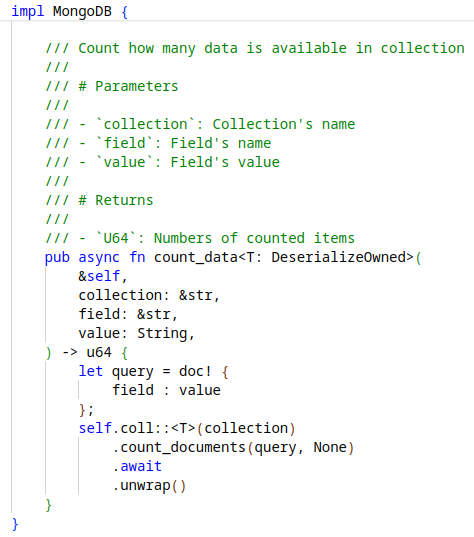
\includegraphics[keepaspectratio, width=12cm]{gambar/util-count-data-code.png}
  \caption{Fungsi operasi \emph{count data} dalam \emph{shared utility library}}
  \label{gambar:count-util-code}
\end{figure}

Fungsi \emph{count\_data()} pada gambar \ref{gambar:count-util-code} merupakan fungsi yang digunakan untuk menghintung jumlah data yang dari parameter di dalam \emph{database}. Fungsi ini memiliki 3 parameter, \emph{collection} yang merupakan target \emph{collection} yang akan dihitung datanya, \emph{field} merupakan \emph{field} atau kolom dari data yang akan dihitung, dan \emph{value} adalah value data yang akan dihitung jumlah nya. Fungsi ini mengembalikan nilai yang berbentuk \emph{unsigned integer} yang merupakan jumah data-nya.

\begin{figure}[H]
  \centering
  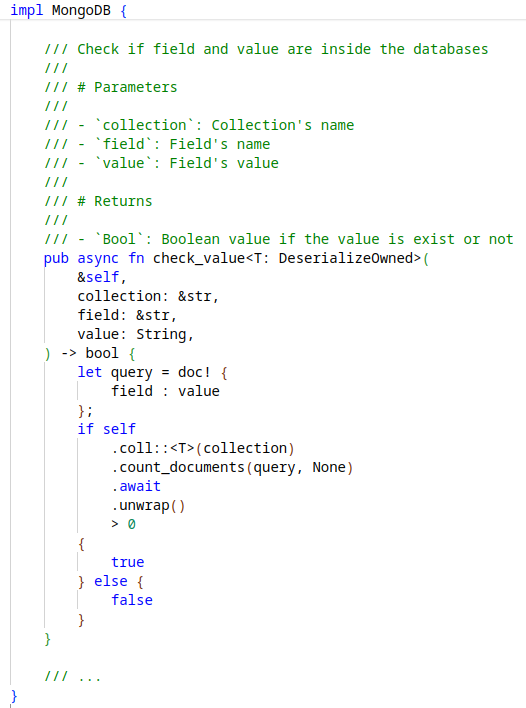
\includegraphics[keepaspectratio, width=12cm]{gambar/util-check-value-code.png}
  \caption{Fungsi operasi \emph{check value} dalam \emph{shared utility library}}
  \label{gambar:checkval-util-code}
\end{figure}

Fungsi \emph{check\_value()} pada gambar \ref{gambar:checkval-util-code} merupakan fungsi yang digunakan untuk mengecek dalam \emph{collection} apakah data yang di deskripsikan ada atau tidak. Parameter dari fungsi ini ada 3 yaitu \emph{collection}, \emph{field}, dan \emph{value}, fungsi ini akan mengecek apakah data dengan \emph{field} dan \emph{value} yang didefinisikan dalam parameter ada atau tidak dalam \emph{collection}. Fungsi ini akan mengembalikan bentuk data \emph{boolean} yang menunjukkan apakah data ini ada atau tidak. Gambar \ref{gambar:function-call} merupakan gambaran dimana fungsi-fungsi ini dipanggil dan berinteraksi dengan \emph{service} apa.

\begin{figure}[H]
  \centering
  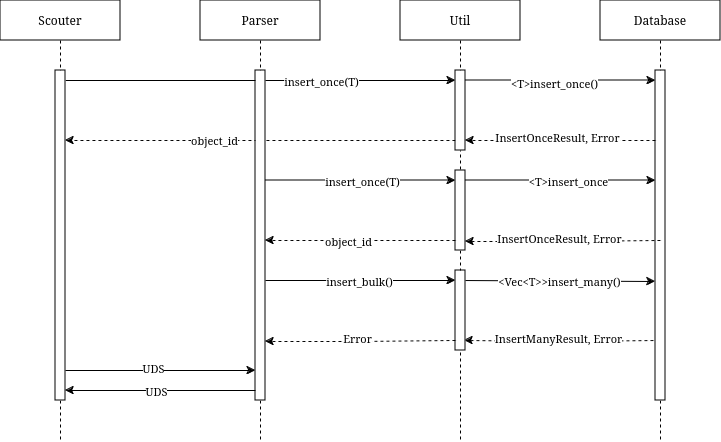
\includegraphics[keepaspectratio, width=13cm]{gambar/function-call-diagram.png}
  \caption{Diagram pemanggilan fungsi dari \emph{shared library onecrawl-util}}
  \label{gambar:function-call}
\end{figure}

Selain fungsi untuk menjalankan \emph{query}, \emph{library} ini juga menyimpan definisi \emph{class} dari \emph{collection} untuk penyimpanan data tersebut. Seluruh definisi ini disimpan dalam \emph{onecrawl-util} untuk meminimalisir kompleksitas dan mempermudah akses terhadap \emph{class} dari semua \emph{services}. Objek dari \emph{class - class} ini yang nantinya akan digunakan sebagai definisi data yang akan disimpan kedalam database. Kode dalam gambar \ref{gambar:struct-page-info} merupakan definisi \emph{class} dari \emph{collection page\_information} dalam \emph{database}. 

\begin{figure}[H]
  \centering
  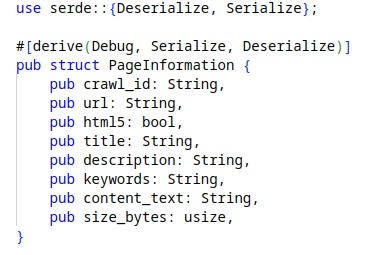
\includegraphics[keepaspectratio, width=10cm]{gambar/struct-page-information.png}
  \caption{Definisi struktur dari objek \emph{PageInformation}}
  \label{gambar:struct-page-info}
\end{figure}

Semua deifinisi \emph{class} ini disimpan dalam file \emph{model.rs} dalam \emph{directory} yang memiliki nama yang sesuai dengan nama \emph{collectionnya}, dan semua \emph{class} ini di abstraksikan sehingga dapat diakses dari file \emph{monggodb.rs}.

\begin{figure}[H]
  \centering
  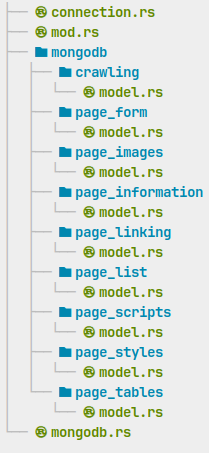
\includegraphics[keepaspectratio, width=4cm]{gambar/file-structure-db-util.png}
  \caption{Struktur \emph{file} dan \emph{folder} dari \emph{database model}}
  \label{gambar:file-structure-db-util}
\end{figure}

\subsection{Pencarian \emph{multi-column}}

\begin{figure}[H]
  \centering
  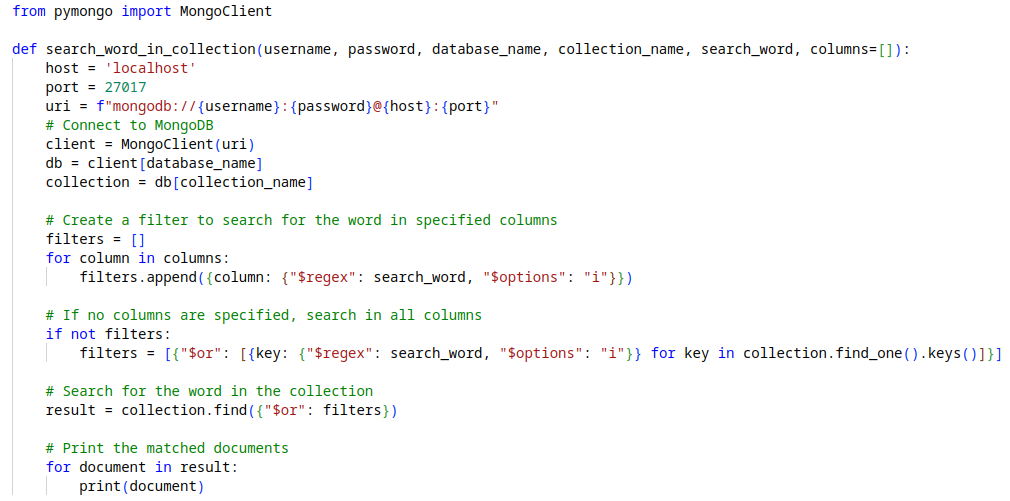
\includegraphics[keepaspectratio, width=14cm]{gambar/onequery-code.png}
  \caption{Fungsi untuk melakukan \emph{multi-column} search}
  \label{gambar:onequery-code}
\end{figure}

\section{Pengujian \emph{Web Crawler} }

Proses pengujian \emph{web crawler} akan difokuskan pada 3 sisi yaitu jumlah halaman web terkumpul, persebaran \emph{domain} web, dan \emph{resource} terpakai saat \emph{crawler} berjalan terutama \emph{cpu usage} dan \emph{memory usage}.

\subsection{Pengujian Jumlah Halaman Web Tersimpan}

Pada penelitian ini pengujian dilakukan pada 3 \emph{origin url} yaitu "https://detik.com", "https://kompas.com", dan "https://bola.com". Pengujian dilakukan selama 2 jam atau 7200 detik dan menggunakan maksimum 5 \emph{threads}. 

\begin{table}[H]
  \caption{Perbandingan jumlah \emph{row} dari halaman web yang terunnduh}
  \begin{center}
    \begin{tabular}{ |p{5cm}|p{3cm}| } \hline
      \textbf{Jenis \emph{crawler}}& \textbf{Total rows} \\ \hline
      \emph{Old Crawler}&  2900 \\ \hline
      \emph{New Crawler}& 50818 \\ \hline
    \end{tabular}
  \end{center}
\end{table}

Dari jumlah total hasil halaman yang berhasil tersimpan terdapat kenaikan sebesar 17x atau 1700 persen kenaikan jumlah halaman terkumpul.

\subsection{Pengujian Persebaran \emph{Domain} dari halaman web tersimpan}

Aspek lain yang diuji dari \emph{crawler} adalah persebaran antara domain yang berhasi terkumpul.

\begin{table}[H]
  \caption{Persebaran domain dari keseluruhan halaman web yang terunduh}
  \begin{center}
    \begin{tabular}{ |p{3.5cm}|p{3.5cm}|p{3.5cm}| } \hline
      \textbf{https://detik.com}& \textbf{https://kompas.com}& \textbf{https://bola.net} \\ \hline
      38368& 8839& 3611 \\ \hline
    \end{tabular}
  \end{center}
\end{table}

\subsection{Pengujian \emph{language tree durability}}

Untuk menguji proses pembangunan \emph{language tree} dari \emph{crawler} ini, dilakukan proses \emph{crawling} pada dua halaman web dengan struktur yang berbeda untuk membandingkan informasi yang di dapatkan. Pengujian dilakukan terhadap dua halaman web dari domain berita \emph{detik.com} dan domain blog \emph{kaskus.co.id}.

Dari domain \emph{detik.com} halaman yang diuji adalah \emph{https://www.kompas.com/food/read/2024/03/24/111100775/6-cara-bikin-telur-dadar-padang-mengembang-tinggi-ala-restoran}. Dari halaman web ini didapatkan informasi \emph{page\_information sebagai berikut},

\begin{figure}[H]
  \centering
  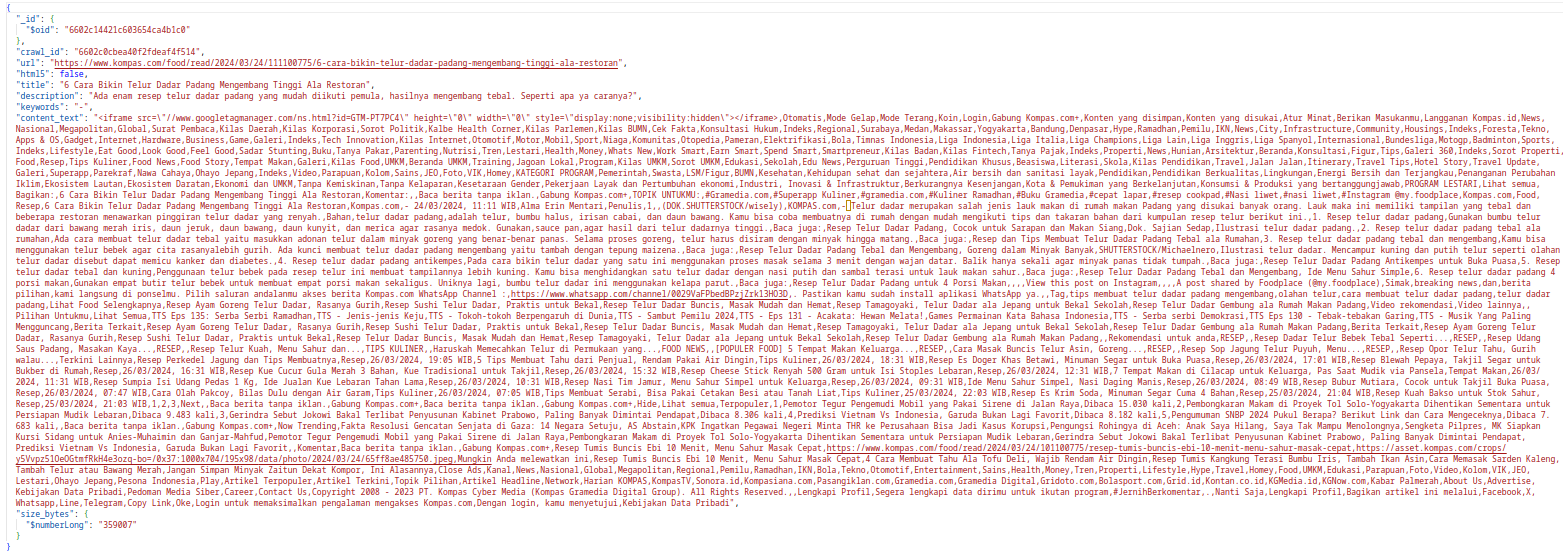
\includegraphics[keepaspectratio, width=14cm]{gambar/detik-bench-pageinfo.png}
  \caption{Konten dari halaman web \emph{detik.com} yang terunduh}
  \label{gambar:detik-bench-pageinfo}
\end{figure}

Teks kontent yang berhasil dikumpulkan dari halaman web ini berjumlah 1650 kata, selain itu dari halaman tersebut juga terkumpul 20 \emph{outbound url}

Untuk domain \emph{kaskus.co.id}, halaman yang diuji adalah \emph{https://www.kaskus.co.id/thread/6609ee1ced160346e4016557/boikot-black-armada-dubes-australia-australia-pendukung-terkuat-republik-indonesia}. Informasi yang dikumpulkan dalam \emph{page\_information} adalah,

\begin{figure}[H]
  \centering
  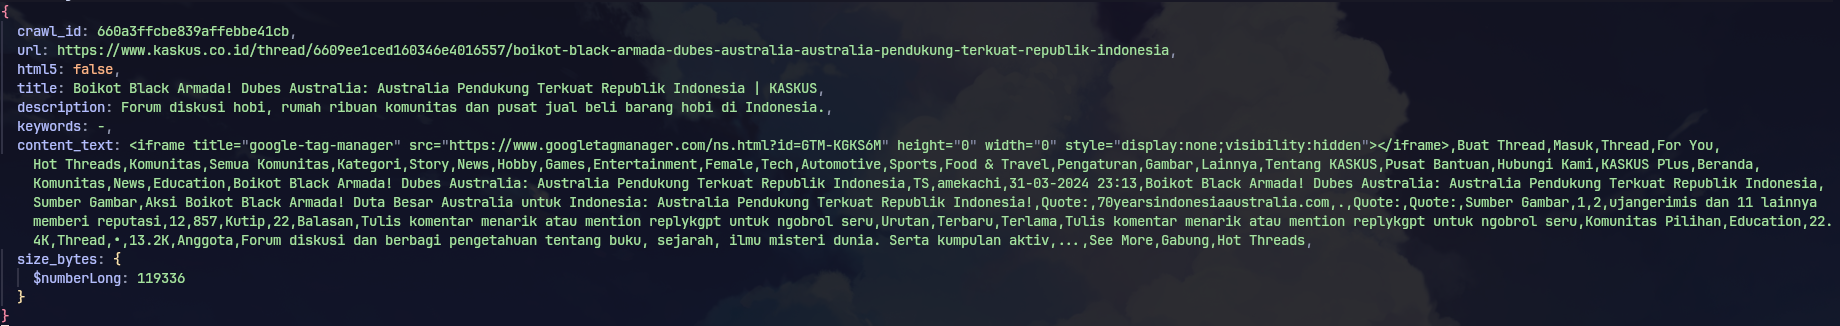
\includegraphics[keepaspectratio, width=14cm]{gambar/kaskus-bench-pageinfo.png}
  \caption{Konten dari halaman web \emph{kaskus.id} yang terunduh}
  \label{gambar:kaskus-bench-pageinfo}
\end{figure}

Teks konten yang berhasil dikumpulkan berjumlah 82 kata, dengan 19 \emph{outbound url} yang terkumpul.

\subsection{Pengujian Penggunan \emph{CPU Resource}}

Pengukuran penggunaan \emph{cpu resource} menggunakan metode \emph{perf record} dimana pengukuran dilakukan terhadap \emph{core cycyle} atau berapa banyak suatu objek dijalankan oleh \emph{cpu}, ini akan menunjukkan seberapa besar penggunaan \emph{resource} suatu objek relatif terhadap penggunaan \emph{resource} dari keseluruhan \emph{crawler}. Hasil dari pengukuran ditunjukkan dalam bentuk \emph{bar graph}. Berikut merupakan hasil pengukurang \emph{cpu resource} dari kedua \emph{services},

\begin{figure}[H]
  \centering
  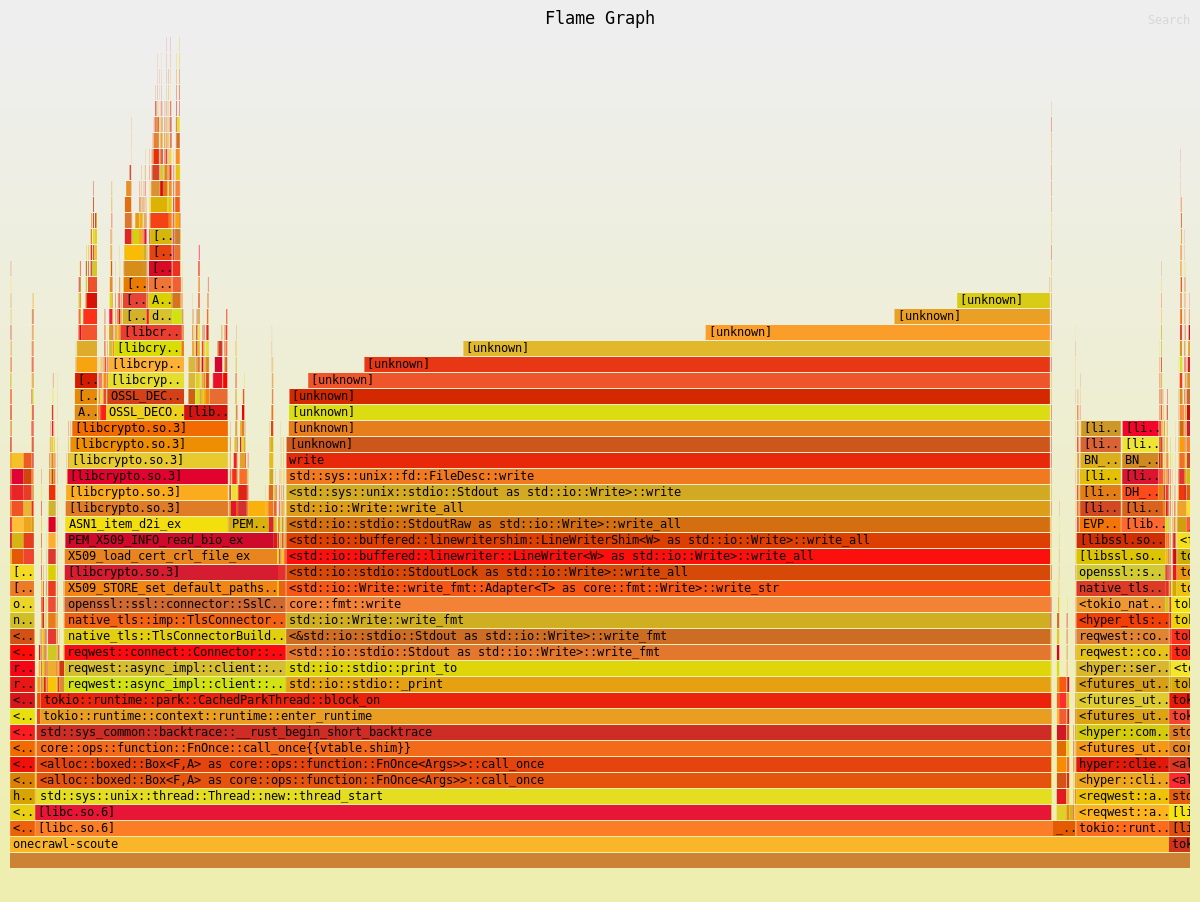
\includegraphics[keepaspectratio, width=14cm]{gambar/graph/cpu-bench-parser.png}
  \caption{Pengunaan \emph{cpu resource} \emph{crawler}}
  \label{gambar:cpu-bench-parser}
\end{figure}

Dari diagram dalam gambar \ref{gambar:cpu-bench-parser} dapat di lihat bahwa, penggunaan \emph{cpu resource} terbanyak dilakukan oleh \emph{tokio} sebagai \emph{manager runtime} dari \emph{multi-threading} dan mekanisme \emph{async} yang digunakan oleh kedua \emph{services}.

\subsection{Pengujian Penggunan \emph{Memory Resource}}

Dalam pengujian penggunaan \emph{memory resource} \emph{crawler}, penggunaan \emph{memory} dari dua service dipantau selama jalannya proses \emph{crawling}. Terdapat 3 data yang dipantau dalam pengujian yaitu, 

\begin{enumerate}
  \item{\emph{Memory Allocated}. Total alokasi \emph{memory}}
  \item{\emph{Memory Allocated (never  deallocated)}. Alokasi \emph{memory} yang tidak pernah di dealokasi}
  \item{\emph{Total Usage}. Jumlah total penggunaan \emph{Memory}}
\end{enumerate}

Berikut merupakan hasil \emph{graph} penggunaan \emph{memory} dari \emph{scouter service},

\begin{figure}[H]
  \centering
  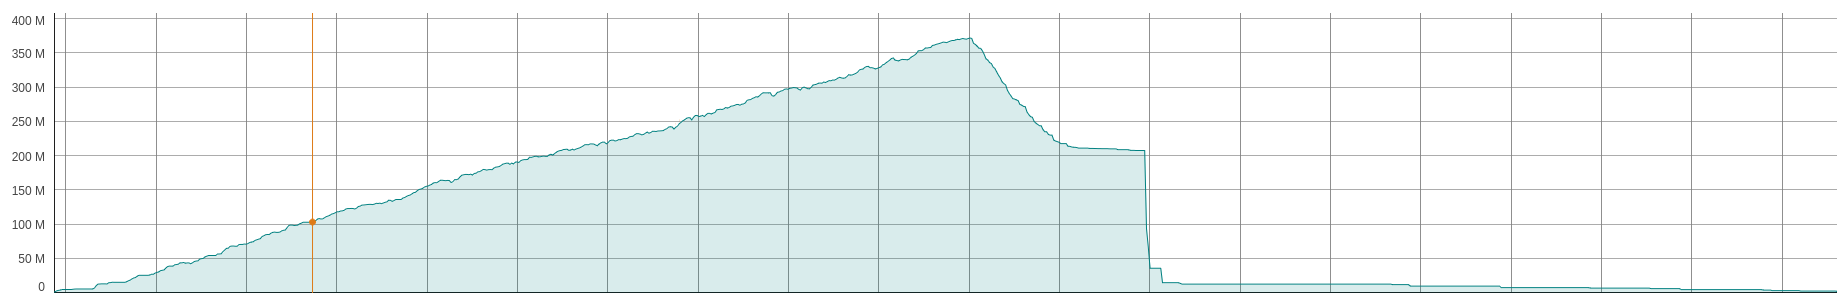
\includegraphics[keepaspectratio, width=15cm]{gambar/graph/scouter-total-alloc.png}
  \caption{Total alokasi \emph{memory}}
  \label{gambar:scouter-total-alloc}
\end{figure}

Graph dari gambar \ref{gambar:scouter-total-alloc} Menunjukkan alokasi \emph{memory} mentah dihitung per iterasi waktu, dari graph tersebut dapat dilihat alokasi memory tertinggi dari jalannya program \emph{scouter service} adalah 350 Mb.

\begin{figure}[H]
  \centering
  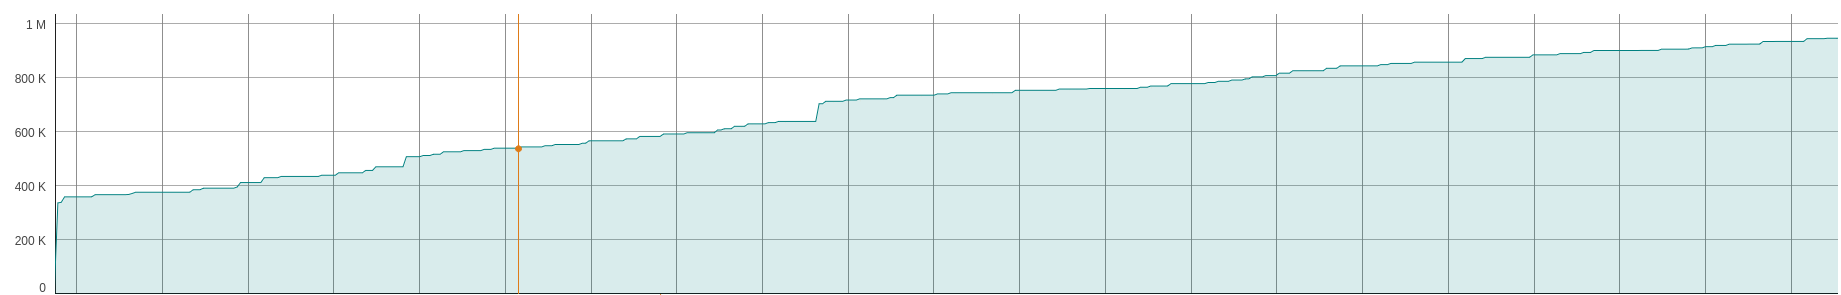
\includegraphics[keepaspectratio, width=15cm]{gambar/graph/scouter-never-dealloc.png}
  \caption{\emph{memory} yang tidak di dealokasi}
  \label{gambar:scouter-never-dealloc}
\end{figure}

Sedangkan gambar \ref{gambar:parser-never-dealloc} menunjukkan jumlah memori teralokasi yang tidak di bebaskan oleh program, graph ini menunjukkan jumlah \emph{memory} yang bocor atau \emph{memory leak} dari program. Dari graph dapat diidentifikasi terdapat \emph{memory leak} dengan jumlah maksimal 1 Mb.

\begin{figure}[H]
  \centering
  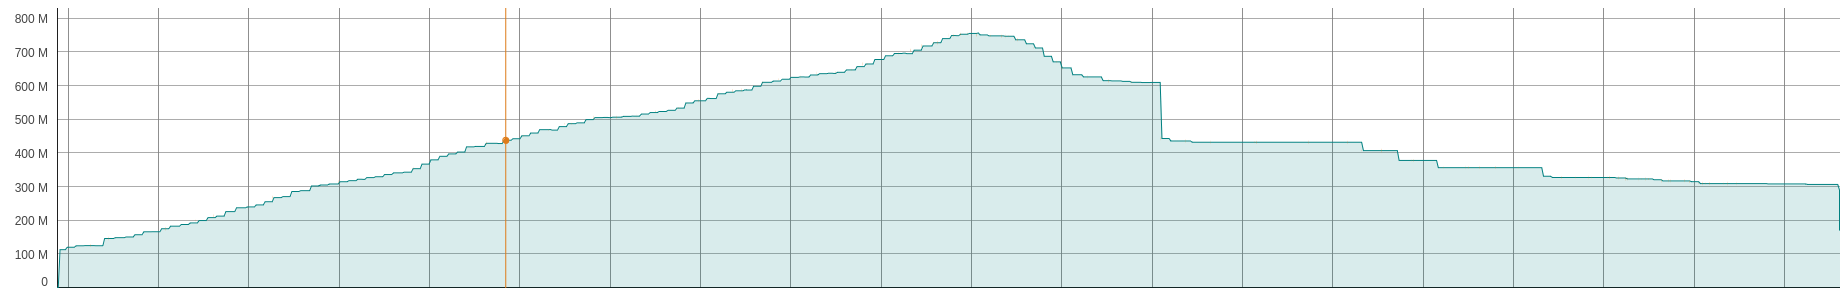
\includegraphics[keepaspectratio, width=15cm]{gambar/graph/scouter-total-usage.png}
  \caption{Total penggunaan \emph{memory}}
  \label{gambar:scouter-total-usage}
\end{figure}

Sedangkan graph \ref{gambar:scouter-total-alloc} menunjukkan total penggunaan memory yang di alokasi dikurang memory yang berhasil dibebaskan, dari graph tersebut dapat di ungkap bahwa total penggunaan memory paling tinggi dari \emph{scouter} adalah sejumlah 700 Mb.

Berikut merupakan hasil \emph{graph} penggunaan \emph{memory} dari \emph{parser service},

\begin{figure}[H]
  \centering
  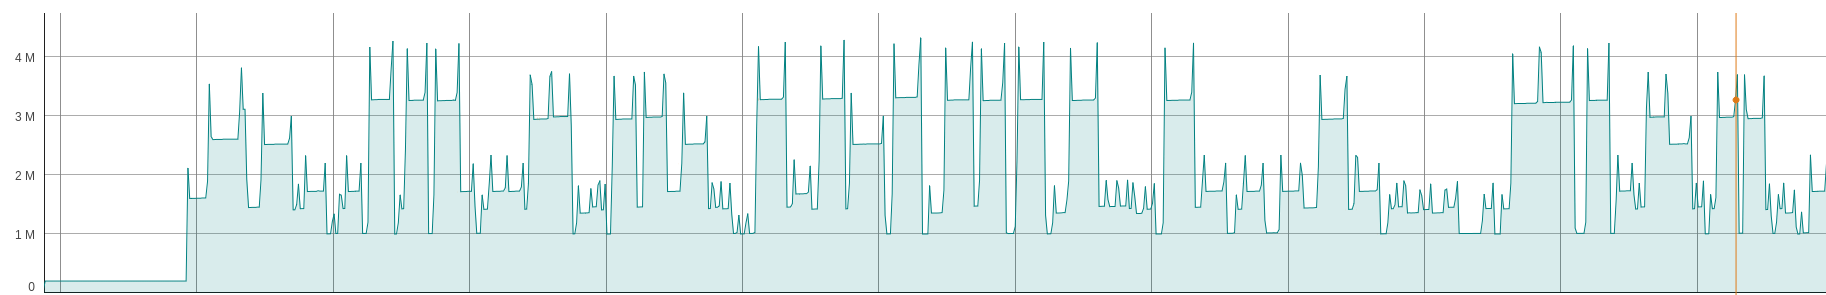
\includegraphics[keepaspectratio, width=15cm]{gambar/graph/parser-total-alloc.png}
  \caption{Total alokasi \emph{memory}}
  \label{gambar:parser-total-alloc}
\end{figure}

\begin{figure}[H]
  \centering
  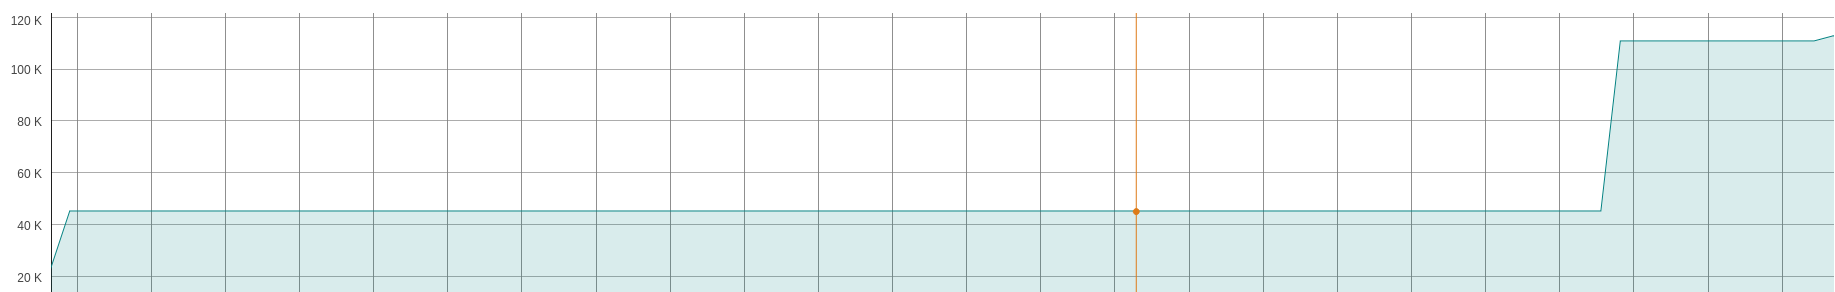
\includegraphics[keepaspectratio, width=15cm]{gambar/graph/parser-never-dealloc.png}
  \caption{\emph{memory} yang tidak di dealokasi}
  \label{gambar:parser-never-dealloc}
\end{figure}

\begin{figure}[H]
  \centering
  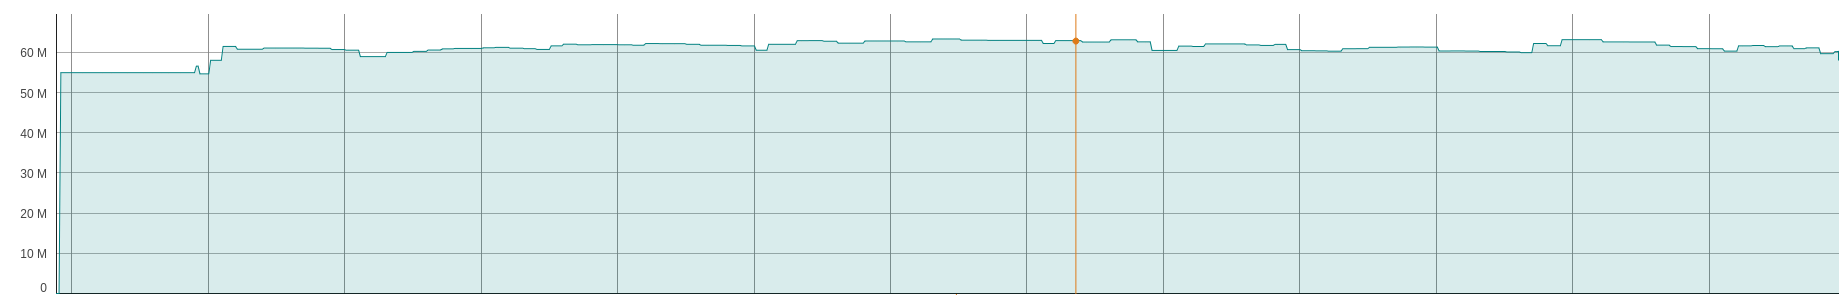
\includegraphics[keepaspectratio, width=15cm]{gambar/graph/parser-total-usage.png}
  \caption{Total penggunaan \emph{memory}}
  \label{gambar:parser-total-usage}
\end{figure}

Ketiga graph dari ketiga gambar diatas menunjukkan bahwa secara rata-rata penggunaan \emph{memory} dari \emph{parser services} lebih rendah dari \emph{scouter}, dengan fluktuasi alokasi yang lebih fluktuatif juga, hal ini dikarenakan \emph{parser} yang tidak memiliki \emph{thread} sebanyak \emph{crawler}.

\subsection{Analisis Hasil}

Berdasarkan data yang telah dikumpulkan, analisis pengujian adalah sebagai berikut,

\begin{enumerate}
  \item Jumlah halaman web yang berhasil dikumpulkan oleh \emph{crawler} dengan waktu dan \emph{origin url} yang sama mencapai 25x dari \emph{crawler} sebelumnya
  \item Persebaran halaman web antar domain masih tidak berimbang dengan domain \emph{detik.com} mengumpulkan 75.5 persen dari keseluruhan halaman web yang terkumpul. 
  \item Algoritma deteksi dan pengambilan informasi dari \emph{language tree} halaman web masih belum optimal untuk mengambil informasi dari halaman web dengan struktur yang berbeda dari halaman web berita online. Terjadi penurunan jumlah teks konten yang terkumpul sebesar 90 persen, hal juga dipengaruhi faktor bentuk blog yang tak memiliki banyak kata-kata tetapi proses ekstraksi data dari halaman web dengan tipe blog belum sempurna.
  \item Penggunaan \emph{memory} \emph{scouter service} selama berjalan secara fluktuatif dengan pengunaan terbesar mencapai 755 Mb dan penggunaan terkecil mencapai 124 Mb. Sedangkan pengunaan \emph{memory} \emph{parser} jauh lebih kecil dengan pengunaan terbesar hanya mencapai 62 Mb.
\end{enumerate}

Hasil dari pengujian dari sisi peforma menunjukkan \emph{crawler} baru mengalami peningkatan yang signifikan dari sisi jumlah halaman web yang berhasil dikumpulkan, tetapi peningkatan ini memiliki hasil yang tidak terduga yaitu besarnya penggunaan \emph{core resource} dan \emph{memory resource} dari sisi \emph{scouter service} dan tidak merata-nya persebaran domain. Tidak akuratnya dari \emph{crawler} diakibatkan algoritma \emph{breadhth-first search} termodifikasi yang digunakan saat ini hanya membatasi \emph{domain} yang dapat di akses tetapi tidak menangani permasalahan pemerataan jumlah antar \emph{domain} yang sudah di-\emph{whitelisted}.

Besar nya penggunaan \emph{resource} disisi \emph{scouter}, berasal dari implementasi \emph{scouter} berasal dari penggunaan \emph{multi-threading} yang berlebihan dan perbaikan kedepannya harus dipertimbangkan selanjutnya.
